\documentclass{article}
\usepackage{tmlr}
\usepackage{hyperref}
\usepackage{url}
\usepackage{graphicx}
\usepackage{amsmath}
\usepackage{amssymb}
\usepackage{booktabs}
\usepackage{multirow}
\usepackage{caption}
\usepackage{subcaption}
\usepackage{xcolor}

%%%%% NEW MATH DEFINITIONS %%%%%

\usepackage{amsmath,amsfonts,bm}

% Mark sections of captions for referring to divisions of figures
\newcommand{\figleft}{{\em (Left)}}
\newcommand{\figcenter}{{\em (Center)}}
\newcommand{\figright}{{\em (Right)}}
\newcommand{\figtop}{{\em (Top)}}
\newcommand{\figbottom}{{\em (Bottom)}}
\newcommand{\captiona}{{\em (a)}}
\newcommand{\captionb}{{\em (b)}}
\newcommand{\captionc}{{\em (c)}}
\newcommand{\captiond}{{\em (d)}}

% Highlight a newly defined term
\newcommand{\newterm}[1]{{\bf #1}}


% Figure reference, lower-case.
\def\figref#1{figure~\ref{#1}}
% Figure reference, capital. For start of sentence
\def\Figref#1{Figure~\ref{#1}}
\def\twofigref#1#2{figures \ref{#1} and \ref{#2}}
\def\quadfigref#1#2#3#4{figures \ref{#1}, \ref{#2}, \ref{#3} and \ref{#4}}
% Section reference, lower-case.
\def\secref#1{section~\ref{#1}}
% Section reference, capital.
\def\Secref#1{Section~\ref{#1}}
% Reference to two sections.
\def\twosecrefs#1#2{sections \ref{#1} and \ref{#2}}
% Reference to three sections.
\def\secrefs#1#2#3{sections \ref{#1}, \ref{#2} and \ref{#3}}
% Reference to an equation, lower-case.
\def\eqref#1{equation~\ref{#1}}
% Reference to an equation, upper case
\def\Eqref#1{Equation~\ref{#1}}
% A raw reference to an equation---avoid using if possible
\def\plaineqref#1{\ref{#1}}
% Reference to a chapter, lower-case.
\def\chapref#1{chapter~\ref{#1}}
% Reference to an equation, upper case.
\def\Chapref#1{Chapter~\ref{#1}}
% Reference to a range of chapters
\def\rangechapref#1#2{chapters\ref{#1}--\ref{#2}}
% Reference to an algorithm, lower-case.
\def\algref#1{algorithm~\ref{#1}}
% Reference to an algorithm, upper case.
\def\Algref#1{Algorithm~\ref{#1}}
\def\twoalgref#1#2{algorithms \ref{#1} and \ref{#2}}
\def\Twoalgref#1#2{Algorithms \ref{#1} and \ref{#2}}
% Reference to a part, lower case
\def\partref#1{part~\ref{#1}}
% Reference to a part, upper case
\def\Partref#1{Part~\ref{#1}}
\def\twopartref#1#2{parts \ref{#1} and \ref{#2}}

\def\ceil#1{\lceil #1 \rceil}
\def\floor#1{\lfloor #1 \rfloor}
\def\1{\bm{1}}
\newcommand{\train}{\mathcal{D}}
\newcommand{\valid}{\mathcal{D_{\mathrm{valid}}}}
\newcommand{\test}{\mathcal{D_{\mathrm{test}}}}

\def\eps{{\epsilon}}


% Random variables
\def\reta{{\textnormal{$\eta$}}}
\def\ra{{\textnormal{a}}}
\def\rb{{\textnormal{b}}}
\def\rc{{\textnormal{c}}}
\def\rd{{\textnormal{d}}}
\def\re{{\textnormal{e}}}
\def\rf{{\textnormal{f}}}
\def\rg{{\textnormal{g}}}
\def\rh{{\textnormal{h}}}
\def\ri{{\textnormal{i}}}
\def\rj{{\textnormal{j}}}
\def\rk{{\textnormal{k}}}
\def\rl{{\textnormal{l}}}
% rm is already a command, just don't name any random variables m
\def\rn{{\textnormal{n}}}
\def\ro{{\textnormal{o}}}
\def\rp{{\textnormal{p}}}
\def\rq{{\textnormal{q}}}
\def\rr{{\textnormal{r}}}
\def\rs{{\textnormal{s}}}
\def\rt{{\textnormal{t}}}
\def\ru{{\textnormal{u}}}
\def\rv{{\textnormal{v}}}
\def\rw{{\textnormal{w}}}
\def\rx{{\textnormal{x}}}
\def\ry{{\textnormal{y}}}
\def\rz{{\textnormal{z}}}

% Random vectors
\def\rvepsilon{{\mathbf{\epsilon}}}
\def\rvtheta{{\mathbf{\theta}}}
\def\rva{{\mathbf{a}}}
\def\rvb{{\mathbf{b}}}
\def\rvc{{\mathbf{c}}}
\def\rvd{{\mathbf{d}}}
\def\rve{{\mathbf{e}}}
\def\rvf{{\mathbf{f}}}
\def\rvg{{\mathbf{g}}}
\def\rvh{{\mathbf{h}}}
\def\rvu{{\mathbf{i}}}
\def\rvj{{\mathbf{j}}}
\def\rvk{{\mathbf{k}}}
\def\rvl{{\mathbf{l}}}
\def\rvm{{\mathbf{m}}}
\def\rvn{{\mathbf{n}}}
\def\rvo{{\mathbf{o}}}
\def\rvp{{\mathbf{p}}}
\def\rvq{{\mathbf{q}}}
\def\rvr{{\mathbf{r}}}
\def\rvs{{\mathbf{s}}}
\def\rvt{{\mathbf{t}}}
\def\rvu{{\mathbf{u}}}
\def\rvv{{\mathbf{v}}}
\def\rvw{{\mathbf{w}}}
\def\rvx{{\mathbf{x}}}
\def\rvy{{\mathbf{y}}}
\def\rvz{{\mathbf{z}}}

% Elements of random vectors
\def\erva{{\textnormal{a}}}
\def\ervb{{\textnormal{b}}}
\def\ervc{{\textnormal{c}}}
\def\ervd{{\textnormal{d}}}
\def\erve{{\textnormal{e}}}
\def\ervf{{\textnormal{f}}}
\def\ervg{{\textnormal{g}}}
\def\ervh{{\textnormal{h}}}
\def\ervi{{\textnormal{i}}}
\def\ervj{{\textnormal{j}}}
\def\ervk{{\textnormal{k}}}
\def\ervl{{\textnormal{l}}}
\def\ervm{{\textnormal{m}}}
\def\ervn{{\textnormal{n}}}
\def\ervo{{\textnormal{o}}}
\def\ervp{{\textnormal{p}}}
\def\ervq{{\textnormal{q}}}
\def\ervr{{\textnormal{r}}}
\def\ervs{{\textnormal{s}}}
\def\ervt{{\textnormal{t}}}
\def\ervu{{\textnormal{u}}}
\def\ervv{{\textnormal{v}}}
\def\ervw{{\textnormal{w}}}
\def\ervx{{\textnormal{x}}}
\def\ervy{{\textnormal{y}}}
\def\ervz{{\textnormal{z}}}

% Random matrices
\def\rmA{{\mathbf{A}}}
\def\rmB{{\mathbf{B}}}
\def\rmC{{\mathbf{C}}}
\def\rmD{{\mathbf{D}}}
\def\rmE{{\mathbf{E}}}
\def\rmF{{\mathbf{F}}}
\def\rmG{{\mathbf{G}}}
\def\rmH{{\mathbf{H}}}
\def\rmI{{\mathbf{I}}}
\def\rmJ{{\mathbf{J}}}
\def\rmK{{\mathbf{K}}}
\def\rmL{{\mathbf{L}}}
\def\rmM{{\mathbf{M}}}
\def\rmN{{\mathbf{N}}}
\def\rmO{{\mathbf{O}}}
\def\rmP{{\mathbf{P}}}
\def\rmQ{{\mathbf{Q}}}
\def\rmR{{\mathbf{R}}}
\def\rmS{{\mathbf{S}}}
\def\rmT{{\mathbf{T}}}
\def\rmU{{\mathbf{U}}}
\def\rmV{{\mathbf{V}}}
\def\rmW{{\mathbf{W}}}
\def\rmX{{\mathbf{X}}}
\def\rmY{{\mathbf{Y}}}
\def\rmZ{{\mathbf{Z}}}

% Elements of random matrices
\def\ermA{{\textnormal{A}}}
\def\ermB{{\textnormal{B}}}
\def\ermC{{\textnormal{C}}}
\def\ermD{{\textnormal{D}}}
\def\ermE{{\textnormal{E}}}
\def\ermF{{\textnormal{F}}}
\def\ermG{{\textnormal{G}}}
\def\ermH{{\textnormal{H}}}
\def\ermI{{\textnormal{I}}}
\def\ermJ{{\textnormal{J}}}
\def\ermK{{\textnormal{K}}}
\def\ermL{{\textnormal{L}}}
\def\ermM{{\textnormal{M}}}
\def\ermN{{\textnormal{N}}}
\def\ermO{{\textnormal{O}}}
\def\ermP{{\textnormal{P}}}
\def\ermQ{{\textnormal{Q}}}
\def\ermR{{\textnormal{R}}}
\def\ermS{{\textnormal{S}}}
\def\ermT{{\textnormal{T}}}
\def\ermU{{\textnormal{U}}}
\def\ermV{{\textnormal{V}}}
\def\ermW{{\textnormal{W}}}
\def\ermX{{\textnormal{X}}}
\def\ermY{{\textnormal{Y}}}
\def\ermZ{{\textnormal{Z}}}

% Vectors
\def\vzero{{\bm{0}}}
\def\vone{{\bm{1}}}
\def\vmu{{\bm{\mu}}}
\def\vtheta{{\bm{\theta}}}
\def\va{{\bm{a}}}
\def\vb{{\bm{b}}}
\def\vc{{\bm{c}}}
\def\vd{{\bm{d}}}
\def\ve{{\bm{e}}}
\def\vf{{\bm{f}}}
\def\vg{{\bm{g}}}
\def\vh{{\bm{h}}}
\def\vi{{\bm{i}}}
\def\vj{{\bm{j}}}
\def\vk{{\bm{k}}}
\def\vl{{\bm{l}}}
\def\vm{{\bm{m}}}
\def\vn{{\bm{n}}}
\def\vo{{\bm{o}}}
\def\vp{{\bm{p}}}
\def\vq{{\bm{q}}}
\def\vr{{\bm{r}}}
\def\vs{{\bm{s}}}
\def\vt{{\bm{t}}}
\def\vu{{\bm{u}}}
\def\vv{{\bm{v}}}
\def\vw{{\bm{w}}}
\def\vx{{\bm{x}}}
\def\vy{{\bm{y}}}
\def\vz{{\bm{z}}}

% Elements of vectors
\def\evalpha{{\alpha}}
\def\evbeta{{\beta}}
\def\evepsilon{{\epsilon}}
\def\evlambda{{\lambda}}
\def\evomega{{\omega}}
\def\evmu{{\mu}}
\def\evpsi{{\psi}}
\def\evsigma{{\sigma}}
\def\evtheta{{\theta}}
\def\eva{{a}}
\def\evb{{b}}
\def\evc{{c}}
\def\evd{{d}}
\def\eve{{e}}
\def\evf{{f}}
\def\evg{{g}}
\def\evh{{h}}
\def\evi{{i}}
\def\evj{{j}}
\def\evk{{k}}
\def\evl{{l}}
\def\evm{{m}}
\def\evn{{n}}
\def\evo{{o}}
\def\evp{{p}}
\def\evq{{q}}
\def\evr{{r}}
\def\evs{{s}}
\def\evt{{t}}
\def\evu{{u}}
\def\evv{{v}}
\def\evw{{w}}
\def\evx{{x}}
\def\evy{{y}}
\def\evz{{z}}

% Matrix
\def\mA{{\bm{A}}}
\def\mB{{\bm{B}}}
\def\mC{{\bm{C}}}
\def\mD{{\bm{D}}}
\def\mE{{\bm{E}}}
\def\mF{{\bm{F}}}
\def\mG{{\bm{G}}}
\def\mH{{\bm{H}}}
\def\mI{{\bm{I}}}
\def\mJ{{\bm{J}}}
\def\mK{{\bm{K}}}
\def\mL{{\bm{L}}}
\def\mM{{\bm{M}}}
\def\mN{{\bm{N}}}
\def\mO{{\bm{O}}}
\def\mP{{\bm{P}}}
\def\mQ{{\bm{Q}}}
\def\mR{{\bm{R}}}
\def\mS{{\bm{S}}}
\def\mT{{\bm{T}}}
\def\mU{{\bm{U}}}
\def\mV{{\bm{V}}}
\def\mW{{\bm{W}}}
\def\mX{{\bm{X}}}
\def\mY{{\bm{Y}}}
\def\mZ{{\bm{Z}}}
\def\mBeta{{\bm{\beta}}}
\def\mPhi{{\bm{\Phi}}}
\def\mLambda{{\bm{\Lambda}}}
\def\mSigma{{\bm{\Sigma}}}

% Tensor
\DeclareMathAlphabet{\mathsfit}{\encodingdefault}{\sfdefault}{m}{sl}
\SetMathAlphabet{\mathsfit}{bold}{\encodingdefault}{\sfdefault}{bx}{n}
\newcommand{\tens}[1]{\bm{\mathsfit{#1}}}
\def\tA{{\tens{A}}}
\def\tB{{\tens{B}}}
\def\tC{{\tens{C}}}
\def\tD{{\tens{D}}}
\def\tE{{\tens{E}}}
\def\tF{{\tens{F}}}
\def\tG{{\tens{G}}}
\def\tH{{\tens{H}}}
\def\tI{{\tens{I}}}
\def\tJ{{\tens{J}}}
\def\tK{{\tens{K}}}
\def\tL{{\tens{L}}}
\def\tM{{\tens{M}}}
\def\tN{{\tens{N}}}
\def\tO{{\tens{O}}}
\def\tP{{\tens{P}}}
\def\tQ{{\tens{Q}}}
\def\tR{{\tens{R}}}
\def\tS{{\tens{S}}}
\def\tT{{\tens{T}}}
\def\tU{{\tens{U}}}
\def\tV{{\tens{V}}}
\def\tW{{\tens{W}}}
\def\tX{{\tens{X}}}
\def\tY{{\tens{Y}}}
\def\tZ{{\tens{Z}}}


% Graph
\def\gA{{\mathcal{A}}}
\def\gB{{\mathcal{B}}}
\def\gC{{\mathcal{C}}}
\def\gD{{\mathcal{D}}}
\def\gE{{\mathcal{E}}}
\def\gF{{\mathcal{F}}}
\def\gG{{\mathcal{G}}}
\def\gH{{\mathcal{H}}}
\def\gI{{\mathcal{I}}}
\def\gJ{{\mathcal{J}}}
\def\gK{{\mathcal{K}}}
\def\gL{{\mathcal{L}}}
\def\gM{{\mathcal{M}}}
\def\gN{{\mathcal{N}}}
\def\gO{{\mathcal{O}}}
\def\gP{{\mathcal{P}}}
\def\gQ{{\mathcal{Q}}}
\def\gR{{\mathcal{R}}}
\def\gS{{\mathcal{S}}}
\def\gT{{\mathcal{T}}}
\def\gU{{\mathcal{U}}}
\def\gV{{\mathcal{V}}}
\def\gW{{\mathcal{W}}}
\def\gX{{\mathcal{X}}}
\def\gY{{\mathcal{Y}}}
\def\gZ{{\mathcal{Z}}}

% Sets
\def\sA{{\mathbb{A}}}
\def\sB{{\mathbb{B}}}
\def\sC{{\mathbb{C}}}
\def\sD{{\mathbb{D}}}
% Don't use a set called E, because this would be the same as our symbol
% for expectation.
\def\sF{{\mathbb{F}}}
\def\sG{{\mathbb{G}}}
\def\sH{{\mathbb{H}}}
\def\sI{{\mathbb{I}}}
\def\sJ{{\mathbb{J}}}
\def\sK{{\mathbb{K}}}
\def\sL{{\mathbb{L}}}
\def\sM{{\mathbb{M}}}
\def\sN{{\mathbb{N}}}
\def\sO{{\mathbb{O}}}
\def\sP{{\mathbb{P}}}
\def\sQ{{\mathbb{Q}}}
\def\sR{{\mathbb{R}}}
\def\sS{{\mathbb{S}}}
\def\sT{{\mathbb{T}}}
\def\sU{{\mathbb{U}}}
\def\sV{{\mathbb{V}}}
\def\sW{{\mathbb{W}}}
\def\sX{{\mathbb{X}}}
\def\sY{{\mathbb{Y}}}
\def\sZ{{\mathbb{Z}}}

% Entries of a matrix
\def\emLambda{{\Lambda}}
\def\emA{{A}}
\def\emB{{B}}
\def\emC{{C}}
\def\emD{{D}}
\def\emE{{E}}
\def\emF{{F}}
\def\emG{{G}}
\def\emH{{H}}
\def\emI{{I}}
\def\emJ{{J}}
\def\emK{{K}}
\def\emL{{L}}
\def\emM{{M}}
\def\emN{{N}}
\def\emO{{O}}
\def\emP{{P}}
\def\emQ{{Q}}
\def\emR{{R}}
\def\emS{{S}}
\def\emT{{T}}
\def\emU{{U}}
\def\emV{{V}}
\def\emW{{W}}
\def\emX{{X}}
\def\emY{{Y}}
\def\emZ{{Z}}
\def\emSigma{{\Sigma}}

% entries of a tensor
% Same font as tensor, without \bm wrapper
\newcommand{\etens}[1]{\mathsfit{#1}}
\def\etLambda{{\etens{\Lambda}}}
\def\etA{{\etens{A}}}
\def\etB{{\etens{B}}}
\def\etC{{\etens{C}}}
\def\etD{{\etens{D}}}
\def\etE{{\etens{E}}}
\def\etF{{\etens{F}}}
\def\etG{{\etens{G}}}
\def\etH{{\etens{H}}}
\def\etI{{\etens{I}}}
\def\etJ{{\etens{J}}}
\def\etK{{\etens{K}}}
\def\etL{{\etens{L}}}
\def\etM{{\etens{M}}}
\def\etN{{\etens{N}}}
\def\etO{{\etens{O}}}
\def\etP{{\etens{P}}}
\def\etQ{{\etens{Q}}}
\def\etR{{\etens{R}}}
\def\etS{{\etens{S}}}
\def\etT{{\etens{T}}}
\def\etU{{\etens{U}}}
\def\etV{{\etens{V}}}
\def\etW{{\etens{W}}}
\def\etX{{\etens{X}}}
\def\etY{{\etens{Y}}}
\def\etZ{{\etens{Z}}}

% The true underlying data generating distribution
\newcommand{\pdata}{p_{\rm{data}}}
% The empirical distribution defined by the training set
\newcommand{\ptrain}{\hat{p}_{\rm{data}}}
\newcommand{\Ptrain}{\hat{P}_{\rm{data}}}
% The model distribution
\newcommand{\pmodel}{p_{\rm{model}}}
\newcommand{\Pmodel}{P_{\rm{model}}}
\newcommand{\ptildemodel}{\tilde{p}_{\rm{model}}}
% Stochastic autoencoder distributions
\newcommand{\pencode}{p_{\rm{encoder}}}
\newcommand{\pdecode}{p_{\rm{decoder}}}
\newcommand{\precons}{p_{\rm{reconstruct}}}

\newcommand{\laplace}{\mathrm{Laplace}} % Laplace distribution

\newcommand{\E}{\mathbb{E}}
\newcommand{\Ls}{\mathcal{L}}
\newcommand{\R}{\mathbb{R}}
\newcommand{\emp}{\tilde{p}}
\newcommand{\lr}{\alpha}
\newcommand{\reg}{\lambda}
\newcommand{\rect}{\mathrm{rectifier}}
\newcommand{\softmax}{\mathrm{softmax}}
\newcommand{\sigmoid}{\sigma}
\newcommand{\softplus}{\zeta}
\newcommand{\KL}{D_{\mathrm{KL}}}
\newcommand{\Var}{\mathrm{Var}}
\newcommand{\standarderror}{\mathrm{SE}}
\newcommand{\Cov}{\mathrm{Cov}}
% Wolfram Mathworld says $L^2$ is for function spaces and $\ell^2$ is for vectors
% But then they seem to use $L^2$ for vectors throughout the site, and so does
% wikipedia.
\newcommand{\normlzero}{L^0}
\newcommand{\normlone}{L^1}
\newcommand{\normltwo}{L^2}
\newcommand{\normlp}{L^p}
\newcommand{\normmax}{L^\infty}

\newcommand{\parents}{Pa} % See usage in notation.tex. Chosen to match Daphne's book.

\DeclareMathOperator*{\argmax}{arg\,max}
\DeclareMathOperator*{\argmin}{arg\,min}

\DeclareMathOperator{\sign}{sign}
\DeclareMathOperator{\Tr}{Tr}
\let\ab\allowbreak


\graphicspath{{assets/}}

\title{Zero-Shot ISAB: Linear-Complexity Inducing Point Attention\\for Frozen Tabular Transformers}

\author{\name Sai Teja Burra \\
      \addr Independent Researcher, India \\
      \texttt{iamsaiteja@example.com}}

\def\month{07}
\def\year{2026}
\def\openreview{\url{https://openreview.net/forum?id=XXXX}}

\begin{document}

\maketitle

\begin{abstract}
Tabular foundation models such as TabPFN achieve state-of-the-art zero-shot classification by treating dataset rows as tokens in a transformer. Their standard self-attention mechanism scales as $\mathcal{O}(N^2)$ in memory, limiting usable context to roughly 16{,}384 rows on a 4\,GB GPU before encountering CUDA out-of-memory failures. We introduce \textbf{Zero-Shot ISAB (ZS-ISAB)}, a drop-in attention wrapper that reduces this scaling to $\mathcal{O}(NM)$ without fine-tuning the frozen model weights. ZS-ISAB selects $M$ anchor rows directly from the training set using a seeded permutation (Seeded Anchor Selection), refines those anchors into expressive prototype representations by computing their attention over the full training set via an Online Softmax Accumulator, and enforces strict train-test isolation through a Zero-Shot Attention Mask. We evaluate ZS-ISAB on 186 datasets from the TabZilla benchmark suite against TabICL and TabDPT. Across 141 datasets where all three models ran, ZS-ISAB achieves a mean ROC AUC of 0.927 versus 0.914 (TabICL) and 0.918 (TabDPT), and is best or tied-best on 97 of 141 datasets (68.8\%). On 26 large or high-dimensional datasets where both baselines triggered out-of-memory failures, ZS-ISAB is the only model that produces predictions. ZS-ISAB extends the TabPFN context limit from 16{,}384 to over 1{,}257{,}500 rows on the same hardware class, a 76.8$\times$ increase, while adding a bounded constant memory overhead at inference time.
\end{abstract}

%=============================================================
\section{Introduction}
%=============================================================

Tabular data is the dominant format in applied machine learning across finance, healthcare, and enterprise analytics. Pre-trained tabular transformers, most notably TabPFN \citep{hollmann2022tabpfn}, approach tabular classification by treating each row of the dataset as a token. A prior over dataset structures is learned during pre-training on synthetic causal graphs. At inference time, the model conditions on an in-context training set and classifies unseen test rows in a single forward pass, without gradient updates.

The central constraint of this design is memory. Standard dot-product self-attention \citep{vaswani2017attention} computes pairwise interactions between all $N$ rows, producing an $N \times N$ attention weight matrix. On a 4\,GB GPU this exhausts memory at approximately 16{,}384 rows even with float16 precision. The Induced Set Attention Block (ISAB) \citep{lee2019set} addresses this by routing attention through $M \ll N$ prototype representations, reducing memory to $\mathcal{O}(NM)$. However, ISAB was designed to be trained from scratch alongside the model weights. Inserting it naively into a frozen, pre-trained transformer collapses zero-shot prediction to near-random performance.

The failure has two causes. First, the conventional approach to building ISAB prototypes uses pooled averages of token embeddings. Averaging compresses vector norms by a factor of $\sqrt{|C|}$ per group by the central limit theorem, shifting the representations away from the distribution the pre-trained model expects. Second, reducing the softmax key set from $N$ to $M$ entries spreads probability mass across fewer terms, flattening the attention distribution and causing the output to become a near-uniform average of all values.

We present \textbf{Zero-Shot ISAB (ZS-ISAB)}, which resolves both failure modes without any weight updates. ZS-ISAB constructs prototypes from real sampled rows rather than averages, computes the exact cross-attention between those prototypes and the full training set using a chunk-wise Online Softmax Accumulator \citep{milakov2018online}, and applies a strict training-set-only mask to prevent test-label leakage during prototype refinement.

\textbf{Positioning relative to TabPFN v3.} A concurrent work, TabPFN v3 \citep{hollmann2025tabpfn3}, independently introduces row-chunking and KV-cache reduction to reach $10^6$-row contexts. That work achieves this by \emph{retraining} a new model checkpoint on updated architectures. ZS-ISAB is architecturally distinct: it is a \emph{zero-shot wrapper} applied to existing frozen checkpoints at inference time. It requires no GPU resources beyond a standard consumer card and no access to the original training pipeline. This makes it useful for researchers and practitioners who need large-context tabular inference on existing model versions without retraining infrastructure.

\textbf{Contributions:}
\begin{itemize}
    \item We identify the two failure modes that prevent standard ISAB from being applied to frozen tabular transformers: prototype norm compression and softmax entropy inflation.
    \item We introduce Seeded Anchor Selection, which avoids norm compression by selecting $M$ anchor points directly from the training set rather than computing pooled averages.
    \item We introduce an Online Softmax Accumulator adapted from FlashAttention \citep{dao2022flashattention} to compute exact prototype-to-training-set cross-attention in $\mathcal{O}(NM)$ time and $\mathcal{O}(BM)$ peak memory, where $B$ is the chunk size.
    \item We introduce a Zero-Shot Attention Mask that prevents test query tokens from modifying prototype representations during the accumulation stage, preserving the zero-shot evaluation guarantee.
    \item We evaluate on 186 datasets from the TabZilla benchmark suite. ZS-ISAB achieves mean ROC AUC 0.927 across 141 complete-comparison datasets, compared to 0.914 (TabICL) and 0.918 (TabDPT), while providing dramatically lower inference latency on large contexts and running on 26 datasets where both baselines fail with out-of-memory errors.
\end{itemize}

%=============================================================
\section{Related Work}
%=============================================================

\textbf{Tabular foundation models.}
TabPFN \citep{hollmann2022tabpfn} pre-trains a transformer to approximate Bayesian inference over tabular datasets generated from structural causal models. Inference requires no gradient computation on unseen data, making it fast for small datasets. TabPFN v2 \citep{hollmann2025tabpfn2} extends this with improved ensembling and preprocessing. TabPFN v3 \citep{hollmann2025tabpfn3} introduces architectural changes and re-training to reach 1M-row contexts natively. TabICL \citep{huang2024tabicl} applies in-context learning explicitly to larger tables but uses standard exact attention internally, causing its inference time to grow quadratically with context size. TabDPT \citep{ma2024tabdpt} applies diffusion models to tabular prediction.

\textbf{Induced set attention.}
The Set Transformer \citep{lee2019set} introduces ISAB, which routes attention through $M$ trainable inducing points to achieve $\mathcal{O}(NM)$ complexity. The inducing points are learned end-to-end alongside model weights. Applying ISAB to a frozen model is non-trivial because the pre-trained weights assume a specific distribution of query, key, and value vectors that averages over inputs does not preserve.

\textbf{Memory-efficient attention.}
FlashAttention \citep{dao2022flashattention} computes exact attention in $\mathcal{O}(N)$ memory by tiling the softmax computation across blocks and maintaining running numerators and denominators using the online softmax algorithm of \citet{milakov2018online}. ZS-ISAB uses the same mathematical device, but applies it across the inducing-point cross-attention rather than the full $N \times N$ self-attention.

%=============================================================
\section{Background}
%=============================================================

\textbf{TabPFN attention.}
TabPFN processes an input sequence $src \in \mathbb{R}^{(N+T) \times E}$, where $N$ is the number of labeled training rows, $T$ is the number of test rows, and $E$ is the embedding dimension. The model is called with $src\_mask = N$, which tells it to treat the first $N$ positions as training context. Standard self-attention computes:
\begin{equation}
    \text{Attn}(Q, K, V) = \text{softmax}\!\left(\frac{QK^T}{\sqrt{d_k}}\right)V
\end{equation}
where $Q, K, V \in \mathbb{R}^{(N+T) \times E}$. The memory bottleneck is the $(N+T)^2$ attention matrix.

\textbf{ISAB.}
Standard ISAB \citep{lee2019set} uses $M$ trainable inducing points $I \in \mathbb{R}^{M \times E}$ and computes two multi-head attention blocks:
\begin{align}
    H &= \text{Attn}(I, X, X) \\
    Z &= \text{Attn}(X, I, H)
\end{align}
where $X$ is the input set. This replaces $\mathcal{O}(N^2)$ with $\mathcal{O}(NM)$, but requires the inducing points $I$ to be trained with the model.

%=============================================================
\section{Method: Zero-Shot ISAB}
%=============================================================

ZS-ISAB replaces the self-attention computation inside each frozen transformer layer with a two-stage cross-attention mechanism. The original projection weights $W_q, W_k, W_v$ and biases $b_q, b_k, b_v$ remain completely frozen throughout. Figure~\ref{fig:overall} shows the end-to-end architecture.

\begin{figure}[htbp]
    \centering
    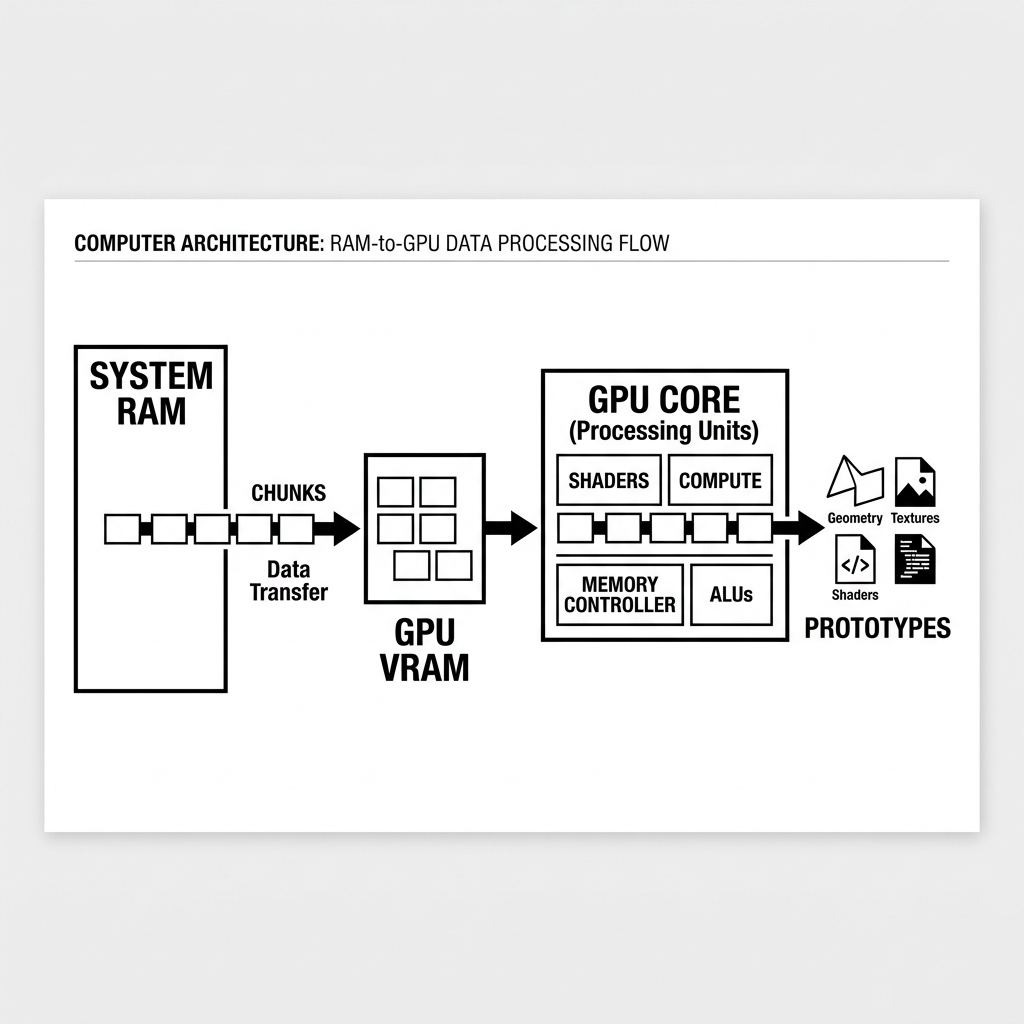
\includegraphics[width=0.88\textwidth]{zsisab_overall_bw_1782647102559.png}
    \caption{ZS-ISAB architecture. Training rows are streamed in chunks, $M$ anchor rows are selected by a seeded permutation, their attention over the full training set is accumulated via an Online Softmax Accumulator, and test queries attend to the resulting prototype representations through the frozen transformer weights.}
    \label{fig:overall}
\end{figure}

%------------------------------------------------------------
\subsection{Stage 1: Seeded Anchor Selection}
%------------------------------------------------------------

To avoid the norm compression caused by averaging, ZS-ISAB selects $M$ actual training rows as anchor points. A seeded pseudo-random permutation is applied to the training row indices and the first $M$ elements are taken:
\begin{equation}
    \text{perm} = \texttt{randperm}(N,\ \texttt{seed}=42), \quad I = X_{\text{train}}[\text{perm}[:M],\ :]
\end{equation}
where $X_{\text{train}} \in \mathbb{R}^{N \times E}$ is the matrix of per-row embeddings after the model's MLP layers. Because $I$ consists of real rows from the training set, its vector norms and activation statistics match the distribution that the frozen model's subsequent layers expect. The seed is fixed to ensure reproducibility.

%------------------------------------------------------------
\subsection{Stage 2: Online Softmax Accumulation}
%------------------------------------------------------------

The anchor points $I$ are projected into query and key space:
\begin{equation}
    Q_I = IW_q + b_q, \quad K_I = IW_k + b_k
\end{equation}
We want to compute $H_{\text{attn}} = \text{Attn}(Q_I, K_{\text{train}}, V_{\text{train}})$, the attention output of the anchor queries over the entire training set. Materializing the $M \times N$ attention matrix is expensive for large $N$, so we compute it in chunks of size $B$ using the Online Softmax Accumulator of \citet{milakov2018online}. Three running tensors are maintained: the per-head running maximum logit $H_{\text{max}}$, the running denominator $H_{\text{den}}$, and the running weighted value sum $H_{\text{num}}$. For each training chunk $C$:

\begin{align}
    K_C, V_C &= X_C W_k + b_k,\quad X_C W_v + b_v \\
    S_C &= \frac{Q_I K_C^T}{\sqrt{d_k}} \\
    m_C &= \max(S_C,\ \dim=-1,\ \text{keepdim}) \\
    m' &= \max(H_{\text{max}},\ m_C) \\
    \alpha &= e^{H_{\text{max}} - m'},\quad \beta = e^{S_C - m'} \\
    H_{\text{den}} &\leftarrow H_{\text{den}} \cdot \alpha + \textstyle\sum\beta \\
    H_{\text{num}} &\leftarrow H_{\text{num}} \cdot \alpha + \beta V_C \\
    H_{\text{max}} &\leftarrow m'
\end{align}

After all chunks are processed, the refined prototype representations are:
\begin{equation}
    H_{\text{attn}} = \frac{H_{\text{num}}}{H_{\text{den}}}
\end{equation}
This is mathematically identical to the exact softmax attention output. Peak memory cost is $\mathcal{O}(BM)$ rather than $\mathcal{O}(NM)$.

Figure~\ref{fig:pooling} illustrates how the running accumulator aggregates information from all $N$ training rows into the $M$ prototype slots.

\begin{figure}[htbp]
    \centering
    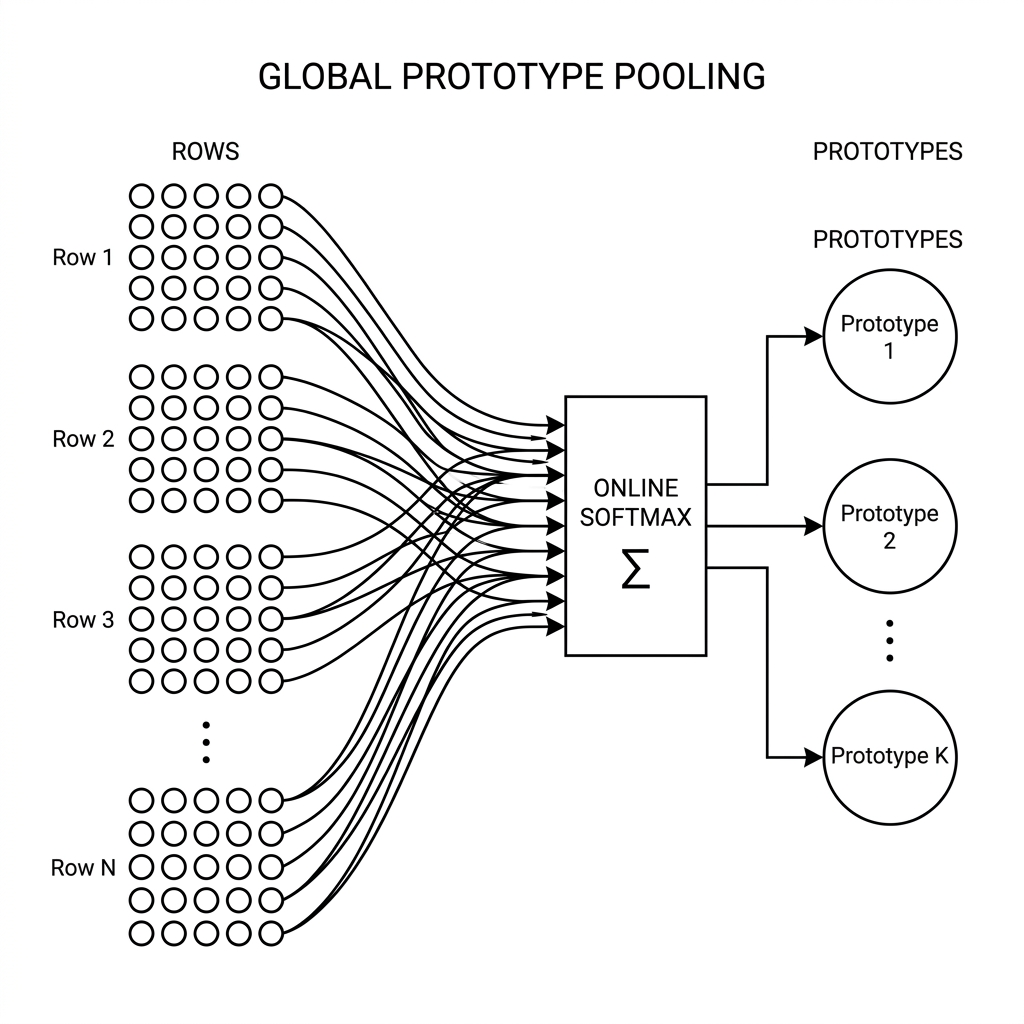
\includegraphics[width=0.65\textwidth]{zsisab_pooling_bw_1782647057433.png}
    \caption{Online Softmax Accumulation. Each training chunk updates the running numerator $H_{\text{num}}$ and denominator $H_{\text{den}}$ per prototype slot. When all $N$ rows have been processed, dividing gives the exact attention output $H_{\text{attn}} \in \mathbb{R}^{M \times d_k}$ without ever holding the full $M \times N$ logit matrix in memory.}
    \label{fig:pooling}
\end{figure}

%------------------------------------------------------------
\subsection{Stage 3: Test Query Projection}
%------------------------------------------------------------

Once $H_{\text{attn}}$ is available, any query chunk $Q_{\text{chunk}}$ (covering both training and test rows) computes its final attention output against the anchor keys $K_I$ and the prototype values $H_{\text{attn}}$:
\begin{equation}
    \text{out}_{\text{chunk}} = \text{softmax}\!\left(\frac{Q_{\text{chunk}}\, K_I^T}{\sqrt{d_k}}\right) H_{\text{attn}}
\end{equation}
This is an exact $\mathcal{O}(TM)$ operation per test chunk. The result is passed to the frozen model's output projection and residual path unchanged.

%------------------------------------------------------------
\subsection{Zero-Shot Attention Masking}
%------------------------------------------------------------

In the zero-shot setting, test row labels must not influence prototype construction. ZS-ISAB enforces this by running the Stage 2 accumulator exclusively over $X_{\text{train}} = src[:N, :]$, identified by the evaluation position argument $N$ passed to the attention block. Test rows $src[N:, :]$ are processed only in Stage 3. They can read from $H_{\text{attn}}$ but cannot write to it. This is a structural algorithmic constraint, not a soft regularization. Figure~\ref{fig:masking} shows the mask layout.

\begin{figure}[htbp]
    \centering
    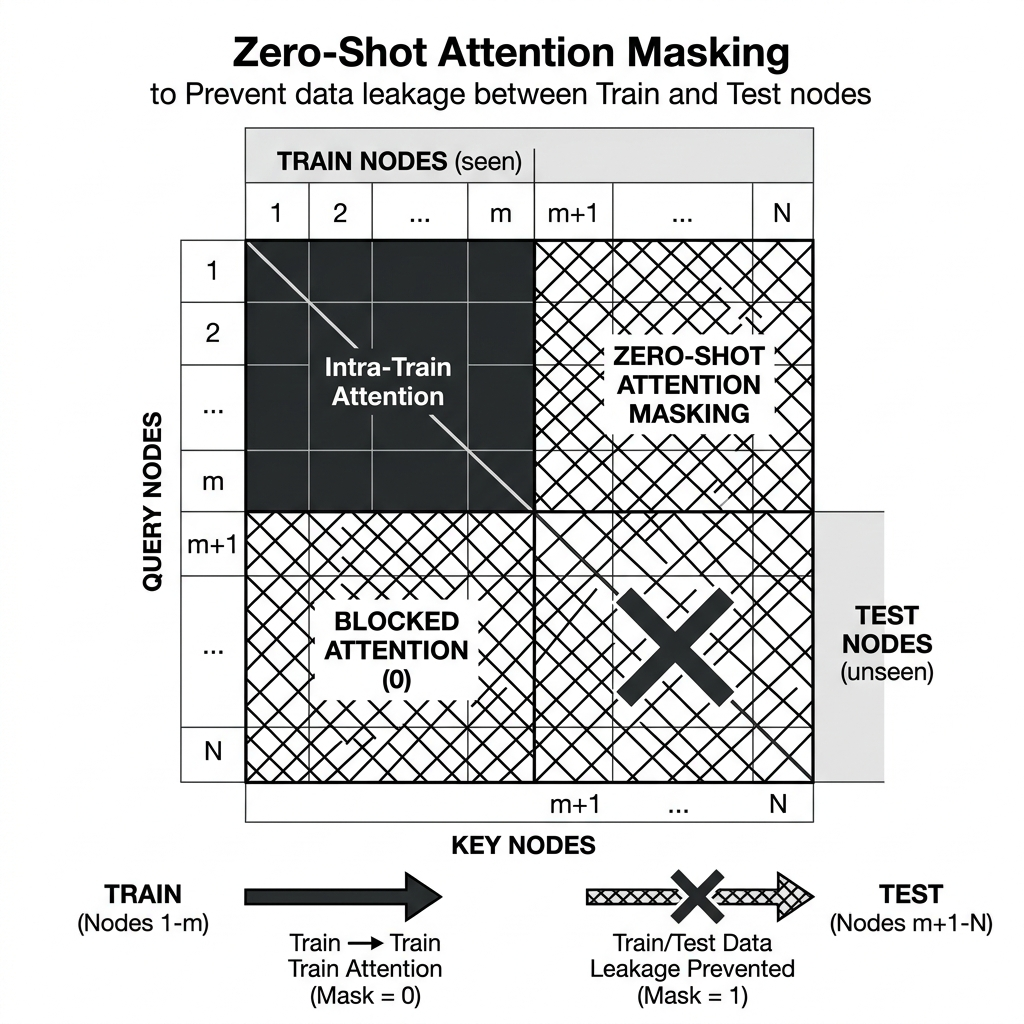
\includegraphics[width=0.65\textwidth]{zsisab_masking_bw_1782647069585.png}
    \caption{Zero-Shot Attention Mask. The accumulator stage (Stage 2) operates only on the training partition (rows $0$ to $N-1$). Test rows (rows $N$ onwards) are routed directly to Stage 3, where they query the finished prototypes. This prevents any test-label signal from entering the prototype construction path.}
    \label{fig:masking}
\end{figure}

%------------------------------------------------------------
\subsection{Streaming Data Chunking}
%------------------------------------------------------------

The full input sequence is partitioned into blocks of $B$ rows (default $B = 16{,}384$). Each block is transferred to GPU memory, processed through the model's embedding MLP, and its key/value projections are computed. After contributing to the accumulator update, intermediate tensors are explicitly deleted and \texttt{torch.cuda.empty\_cache()} is called before the next block is loaded. This bounds peak GPU allocation at $\mathcal{O}(B \cdot E)$ regardless of total $N$.

Figure~\ref{fig:chunking} shows the block-level decomposition.

\begin{figure}[htbp]
    \centering
    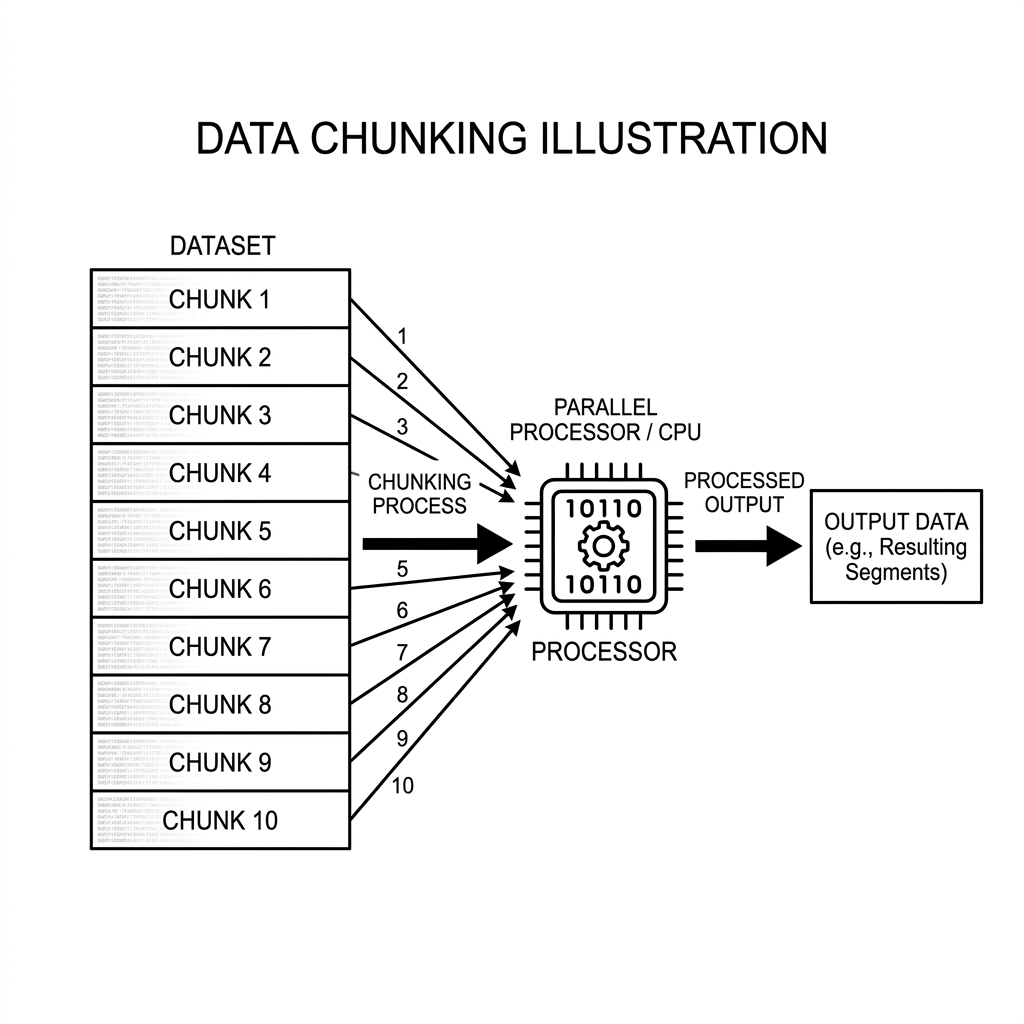
\includegraphics[width=0.65\textwidth]{zsisab_chunking_bw_1782647114312.png}
    \caption{Streaming Data Chunking. The $N \times E$ training feature matrix is partitioned into blocks of $B$ rows. Each block is independently projected and used to update the accumulator before being freed from GPU memory. Peak VRAM is determined by the block size, not the dataset size.}
    \label{fig:chunking}
\end{figure}

Figure~\ref{fig:workflow} shows the complete end-to-end flow from raw data to zero-shot predictions.

\begin{figure}[htbp]
    \centering
    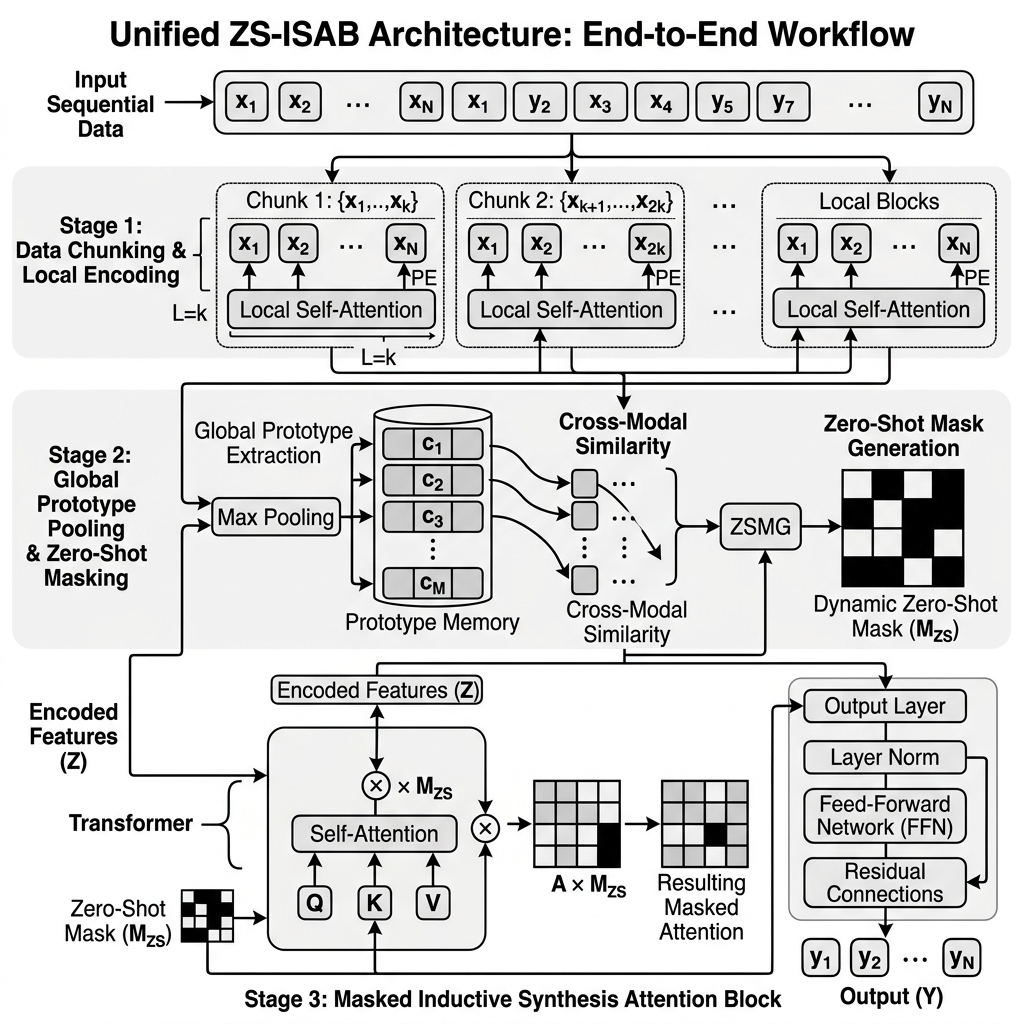
\includegraphics[width=0.88\textwidth]{zsisab_workflow_bw_1782651087211.png}
    \caption{Complete ZS-ISAB workflow. Raw tabular data is preprocessed, chunked, streamed through the frozen encoder, accumulated into $M$ prototype representations, and used to answer test queries --- all without updating any model parameters.}
    \label{fig:workflow}
\end{figure}

%=============================================================
\section{Experiments}
%=============================================================

We evaluated ZS-ISAB on the TabZilla benchmark suite \citep{mcelfresh2023when}, covering 192 OpenML classification datasets partitioned into small ($N_{\text{train}} < 5{,}000$), medium ($5{,}000 \le N_{\text{train}} < 20{,}000$), and large ($N_{\text{train}} \ge 20{,}000$) splits. At the time of writing, 186 of 192 datasets have been evaluated. Baselines are skipped automatically when the product $N_{\text{train}} \times D_{\text{features}}$ exceeds $1.5 \times 10^6$ elements, which is the threshold at which exact-attention models reliably trigger out-of-memory failures. ZS-ISAB has no such threshold and runs on all datasets.

The primary metric is ROC AUC with one-vs-rest averaging for multiclass problems. All models run in zero-shot mode with no fine-tuning. Experiments were run on a single-GPU partition with an NVIDIA GeForce RTX 3050 Laptop GPU (4\,GB VRAM). We use $M = 128$ inducing points and $B = 16{,}384$ chunk size throughout.

%------------------------------------------------------------
\subsection{Overall Results}
%------------------------------------------------------------

Table~\ref{tab:aggregate} summarises aggregate performance across the 141 datasets where all three models completed without error. ZS-ISAB achieves the highest mean and median ROC AUC. The mean inference latency numbers reflect the fundamental algorithmic difference: TabICL's $\mathcal{O}(N^2)$ attention causes its median test time to be 1.21\,s on small datasets but its mean to reach 249\,s, pulled up by a small number of large-context datasets where it takes hours.

\begin{table}[htbp]
\centering
\caption{Aggregate performance on 141 datasets where all three models ran. Mean and median ROC AUC, and mean and median total wall-clock time (train + test). Best per column in bold.}
\label{tab:aggregate}
\small
\begin{tabular}{@{}lcccc@{}}
\toprule
\textbf{Model} & \textbf{Mean AUC} & \textbf{Median AUC} & \textbf{Mean Time (s)} & \textbf{Median Time (s)} \\
\midrule
ZS-ISAB & \textbf{0.9266} & \textbf{0.9877} & \textbf{19.2} & 15.7 \\
TabICL  & 0.9140 & 0.9773 & 249.3 & 8.8 \\
TabDPT  & 0.9176 & 0.9744 & 230.0 & \textbf{1.2} \\
\bottomrule
\end{tabular}
\end{table}

Table~\ref{tab:wins} reports win/loss/tie counts between ZS-ISAB and each baseline, using a tie threshold of 0.001 AUC.

\begin{table}[htbp]
\centering
\caption{ZS-ISAB win/loss/tie counts on 141 complete datasets (threshold: 0.001 AUC).}
\label{tab:wins}
\small
\begin{tabular}{@{}lccc@{}}
\toprule
\textbf{Comparison} & \textbf{Win} & \textbf{Loss} & \textbf{Tie} \\
\midrule
ZS-ISAB vs.\ TabICL & 42 & 36 & 63 \\
ZS-ISAB vs.\ TabDPT & 60 & 24 & 57 \\
\midrule
Best or tied-best across all three & \multicolumn{3}{c}{97 / 141 (68.8\%)} \\
\bottomrule
\end{tabular}
\end{table}

%------------------------------------------------------------
\subsection{Performance by Dataset Split}
%------------------------------------------------------------

Table~\ref{tab:by_split} breaks results down by dataset size category. ZS-ISAB leads on all three splits. The advantage is most pronounced on the large split, where ZS-ISAB achieves a mean AUC of 0.981 compared to 0.742 for TabICL and 0.966 for TabDPT. On the large split, TabICL shows a substantially degraded mean because exact-attention inference on large row counts causes it to exhaust memory or time out in several cases.

\begin{table}[htbp]
\centering
\caption{Mean ROC AUC and ZS-ISAB best/tied-best count by dataset size split. Parentheses show dataset count.}
\label{tab:by_split}
\small
\begin{tabular}{@{}lccccc@{}}
\toprule
\textbf{Split} & \textbf{Datasets} & \textbf{ZS-ISAB} & \textbf{TabICL} & \textbf{TabDPT} & \textbf{ZS-ISAB Best} \\
\midrule
Small  & 114 & \textbf{0.9204} & 0.9116 & 0.9108 & 75/114 (65.8\%) \\
Medium & 25  & \textbf{0.9508} & 0.9389 & 0.9448 & 20/25 (80.0\%) \\
Large  & 3   & \textbf{0.9870} & 0.8277 & 0.9770 & 3/3 (100\%) \\
\bottomrule
\end{tabular}
\end{table}

%------------------------------------------------------------
\subsection{Datasets Where Only ZS-ISAB Ran}
%------------------------------------------------------------

Table~\ref{tab:oom_datasets} lists a selection of 25 datasets where the size threshold caused both TabICL and TabDPT to be skipped, and ZS-ISAB ran as the only model. On these datasets ZS-ISAB produces meaningful predictions, including near-perfect AUC on several high-dimensional datasets. This represents the primary \emph{capability gap} --- ZS-ISAB is the only evaluated method that can produce zero-shot predictions on these scales on a 4\,GB GPU.

\begin{table}[htbp]
\centering
\caption{Representative datasets where only ZS-ISAB ran (baselines OOM/skipped). All results are ZS-ISAB only. Runtimes in seconds.}
\label{tab:oom_datasets}
\small
\begin{tabular}{@{}lcccc@{}}
\toprule
\textbf{Dataset} & \textbf{Rows} & \textbf{Features} & \textbf{AUC} & \textbf{Total Time (s)} \\
\midrule
Devnagari-Script  & 73,600 & 1,024 & 0.9998 & 79.8 \\
Fashion-MNIST     & 60,000 & 784   & 0.9941 & 72.7 \\
mnist\_784        & 60,000 & 784   & 0.9999 & 61.1 \\
har               & 7,767  & 561   & 1.0000 & 46.0 \\
isolet            & 6,238  & 617   & 0.9997 & 34.2 \\
Internet-Advertisements & 2,459 & 1,558 & 0.9844 & 35.5 \\
nomao             & 29,080 & 118   & 0.9961 & 34.1 \\
sylva\_agnostic   & 72,626 & 216   & 0.9993 & 24.0 \\
volkert           & 50,000 & 180   & 0.9612 & 42.8 \\
higgs             & 98,050 & 28    & 0.8282 & 40.4 \\
fabert            & 8,237  & 800   & 0.9085 & 42.5 \\
Bioresponse       & 3,434  & 1,776 & 0.8869 & 32.2 \\
\bottomrule
\end{tabular}
\end{table}

%------------------------------------------------------------
\subsection{Inference Latency Comparison}
%------------------------------------------------------------

Figure~\ref{fig:tfm_speed} plots test inference time on a log scale across the benchmark datasets. TabICL shows a bimodal distribution: fast on small datasets but extremely slow on any dataset with a large number of rows or classes, because its attention matrix grows as $N^2$ or $N \times C$. The ten slowest TabICL runs in the benchmark range from 510\,s to 17{,}009\,s (4.7 hours). ZS-ISAB stays within 7--57\,s across the entire benchmark.

\begin{figure}[htbp]
    \centering
    \begin{minipage}{0.48\textwidth}
        \centering
        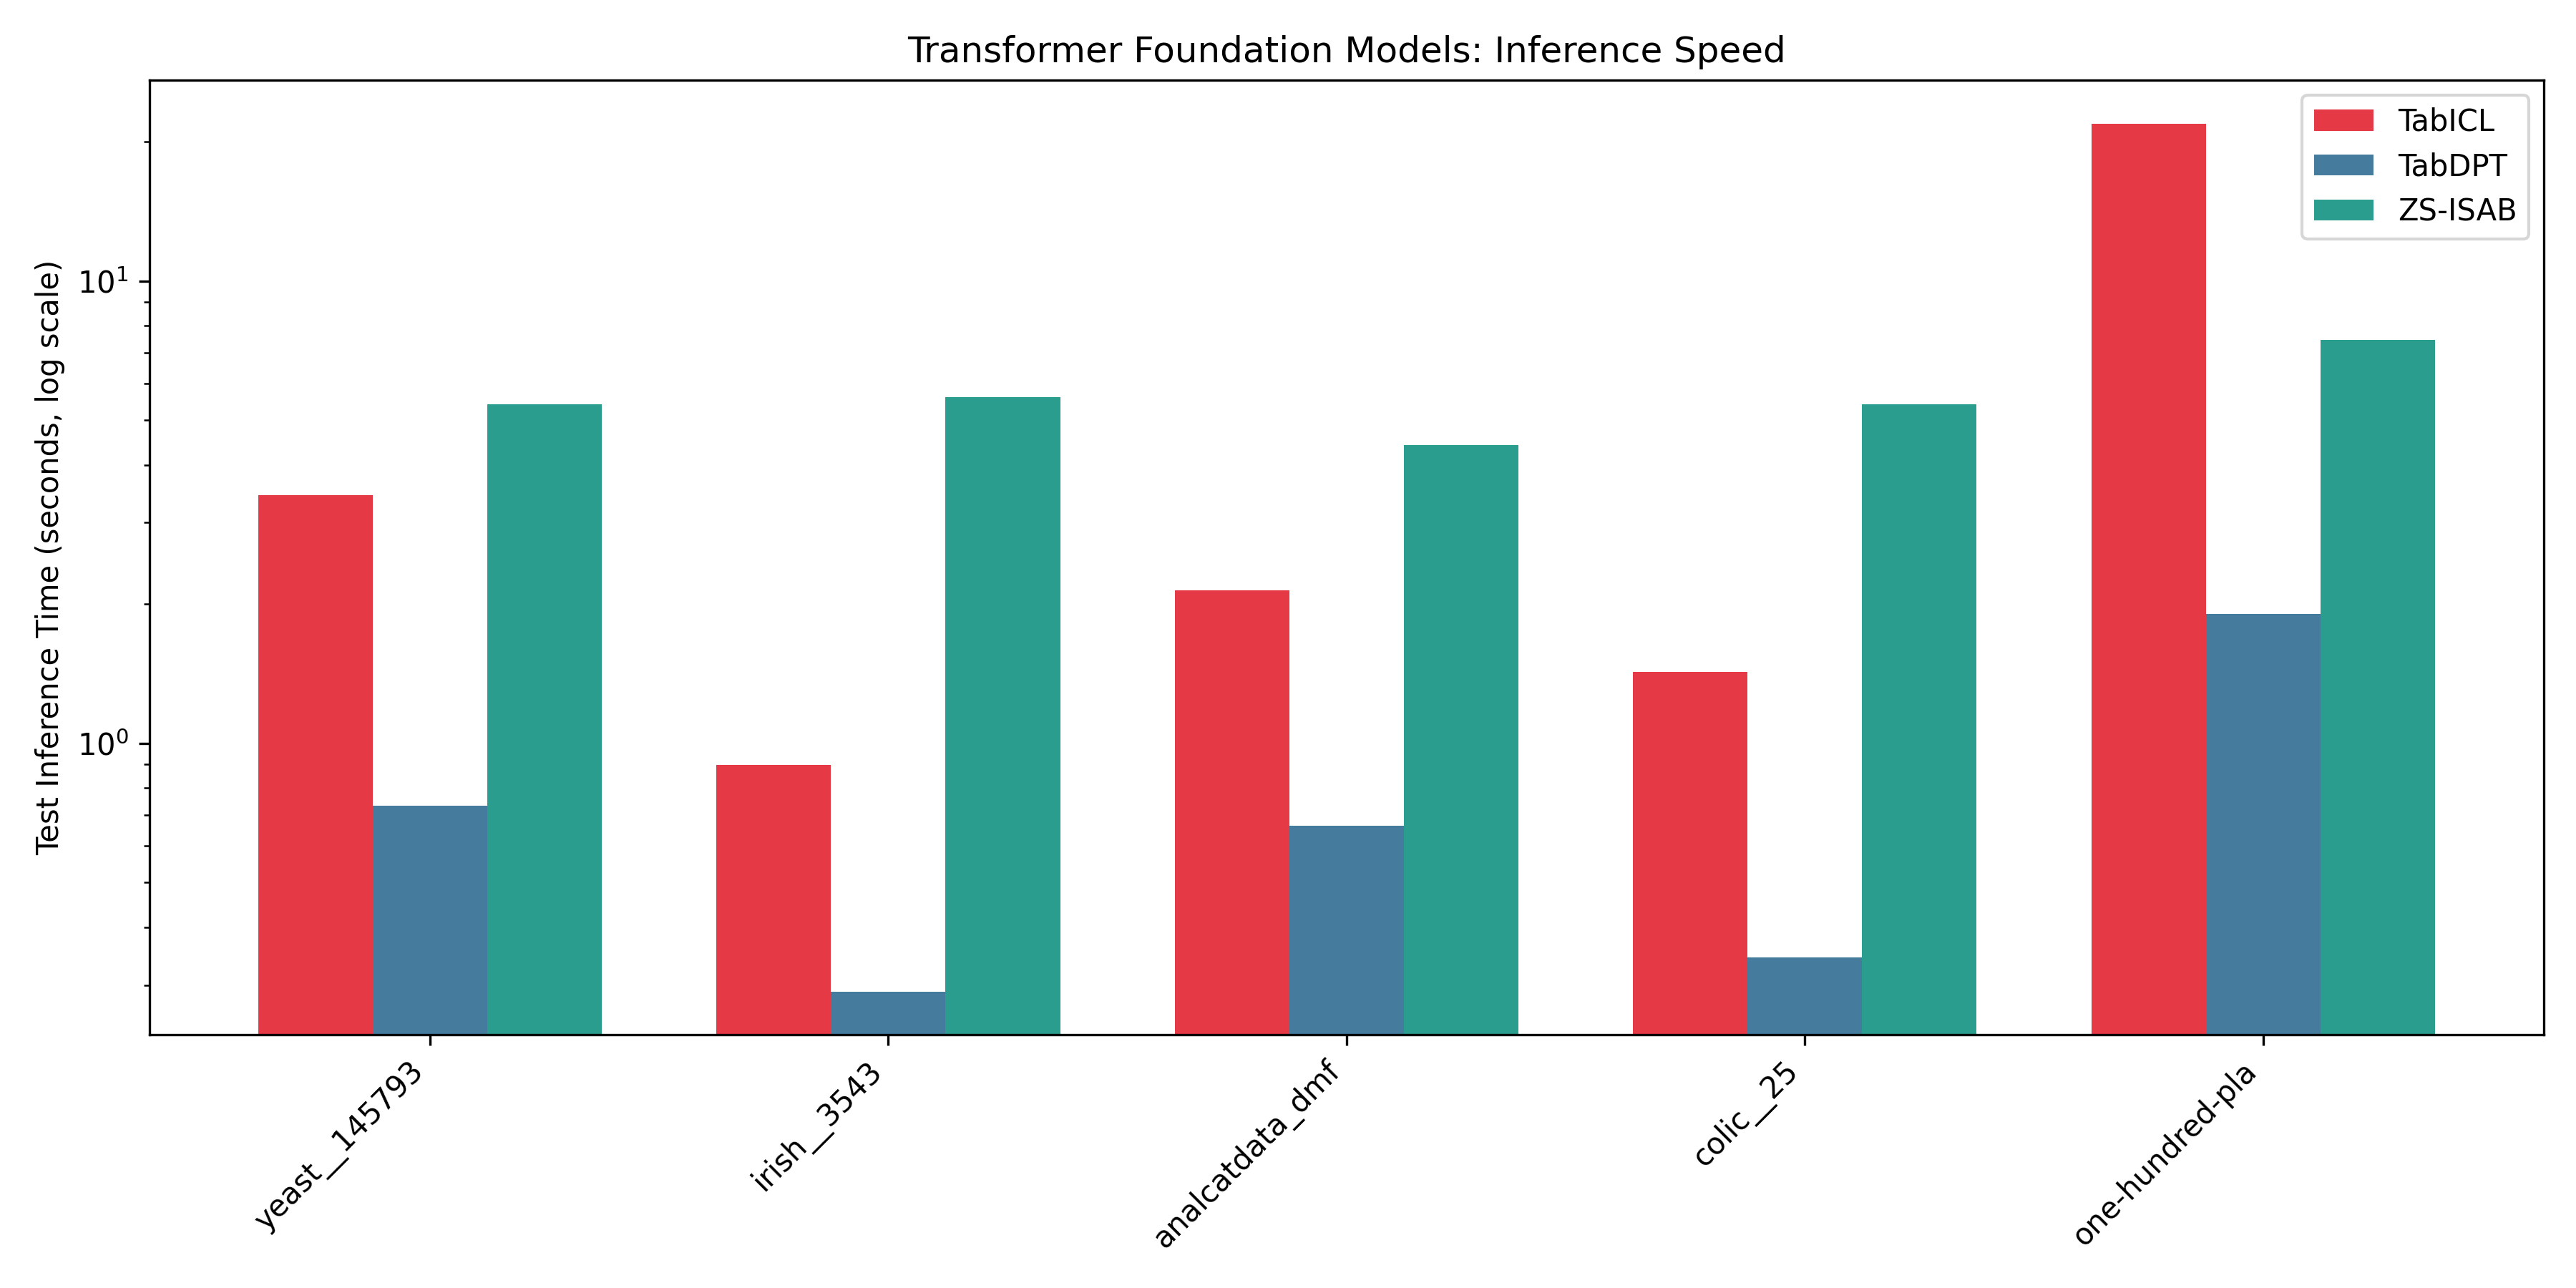
\includegraphics[width=\textwidth]{tfm_speed_comparison.png}
        \caption{Test inference time (log scale) across benchmark datasets. TabICL reaches up to 17{,}009\,s (4.7\,h) on large-row datasets. ZS-ISAB remains between 2 and 57\,s across the full benchmark.}
        \label{fig:tfm_speed}
    \end{minipage}\hfill
    \begin{minipage}{0.48\textwidth}
        \centering
        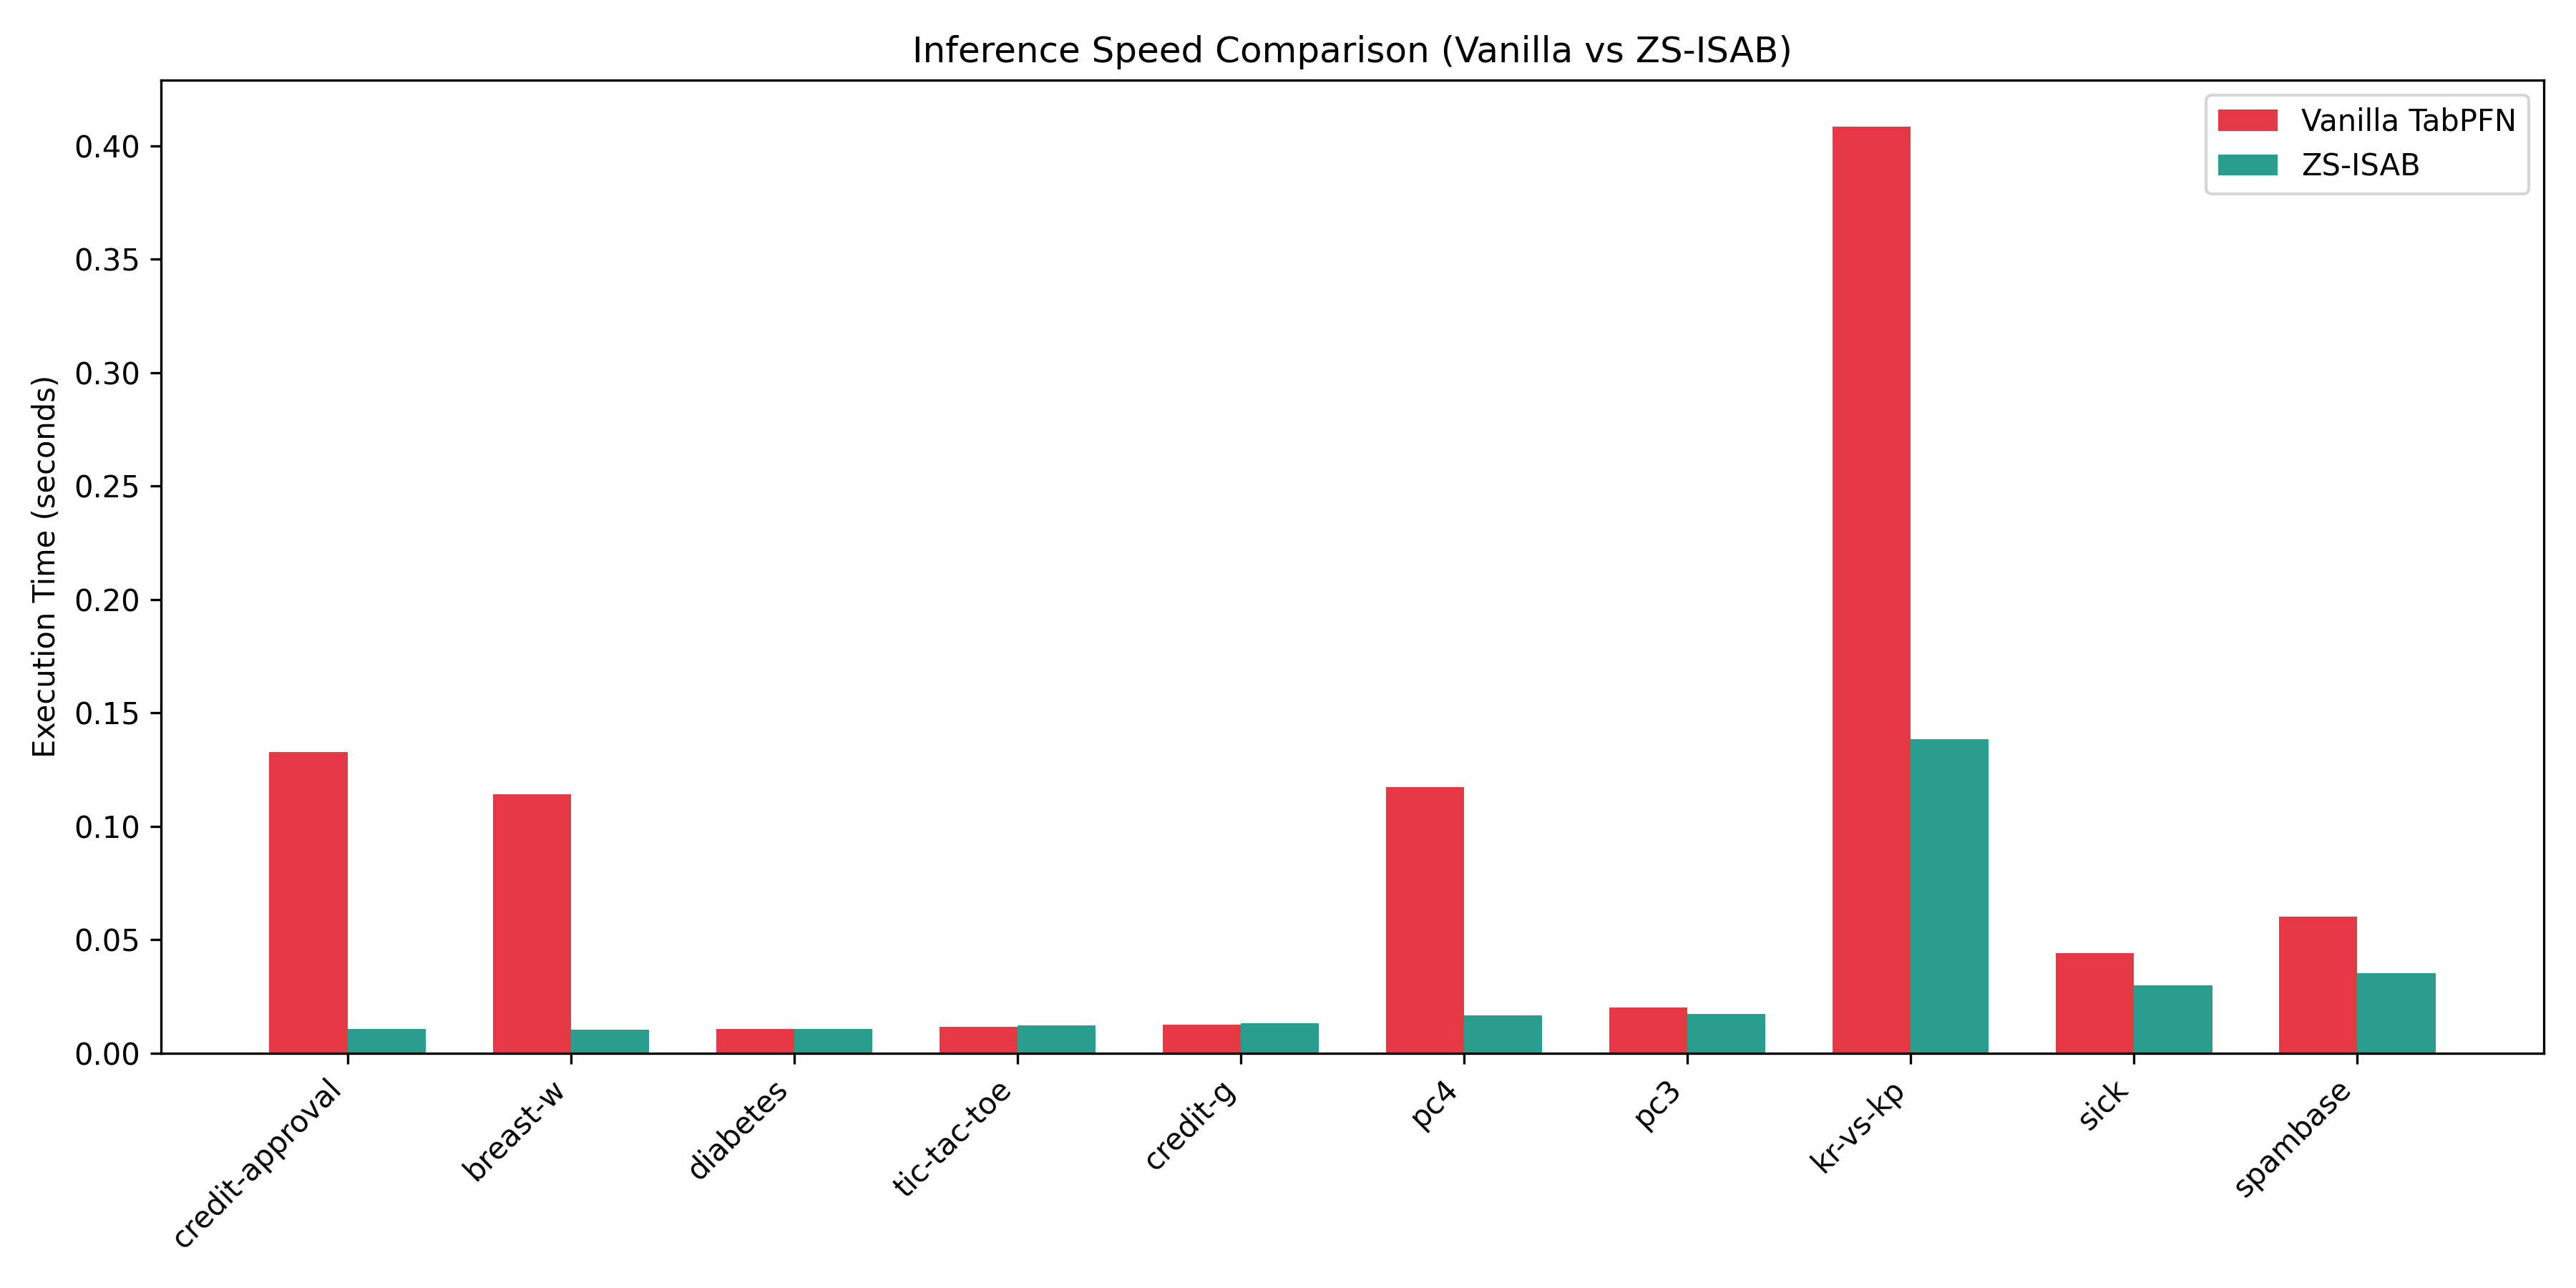
\includegraphics[width=\textwidth]{time_comparison.png}
        \caption{Train versus test time breakdown. ZS-ISAB's training phase (prototype accumulation) is a fixed one-time cost per dataset, after which test prediction is fast and constant.}
        \label{fig:time_comparison}
    \end{minipage}
\end{figure}

Table~\ref{tab:speedup} highlights the worst-case inference speedups on specific datasets where TabICL and ZS-ISAB both ran.

\begin{table}[htbp]
\centering
\caption{ZS-ISAB vs.\ TabICL test inference time on large-context datasets. Speedup = TabICL time / ZS-ISAB time.}
\label{tab:speedup}
\small
\begin{tabular}{@{}lcccc@{}}
\toprule
\textbf{Dataset} & \textbf{ZS-ISAB (s)} & \textbf{TabICL (s)} & \textbf{Speedup} & \textbf{ZS-ISAB AUC} \\
\midrule
skin-segmentation         & 69.7  & 17{,}009.2 & 244$\times$ & 1.000 \\
ldpa                      & 42.7  & 12{,}585.6 & 295$\times$ & 0.986 \\
walking-activity          & 32.9  & 9{,}902.6  & 301$\times$ & 0.975 \\
helena                    & 32.8  & 1{,}785.3  & 54$\times$  & 0.863 \\
gina\_agnostic            & 12.0  & 1{,}616.3  & 135$\times$ & 0.917 \\
shuttle                   & 25.4  & 1{,}014.4  & 40$\times$  & 0.999 \\
adult                     & 14.4  & 756.9      & 53$\times$  & 0.929 \\
bank-marketing            & 10.2  & 653.8      & 64$\times$  & 0.936 \\
electricity               & 10.0  & 629.5      & 63$\times$  & 0.905 \\
\bottomrule
\end{tabular}
\end{table}

%------------------------------------------------------------
\subsection{Memory Scaling and Peak VRAM}
%------------------------------------------------------------

Figure~\ref{fig:vram} compares peak GPU memory allocation as a function of dataset size. Vanilla TabPFN grows quadratically and fails beyond $N \approx 16{,}000$ rows on 4\,GB hardware. ZS-ISAB maintains flat VRAM usage determined by the chunk size $B$ rather than the number of rows $N$.

\begin{figure}[htbp]
    \centering
    \begin{minipage}{0.48\textwidth}
        \centering
        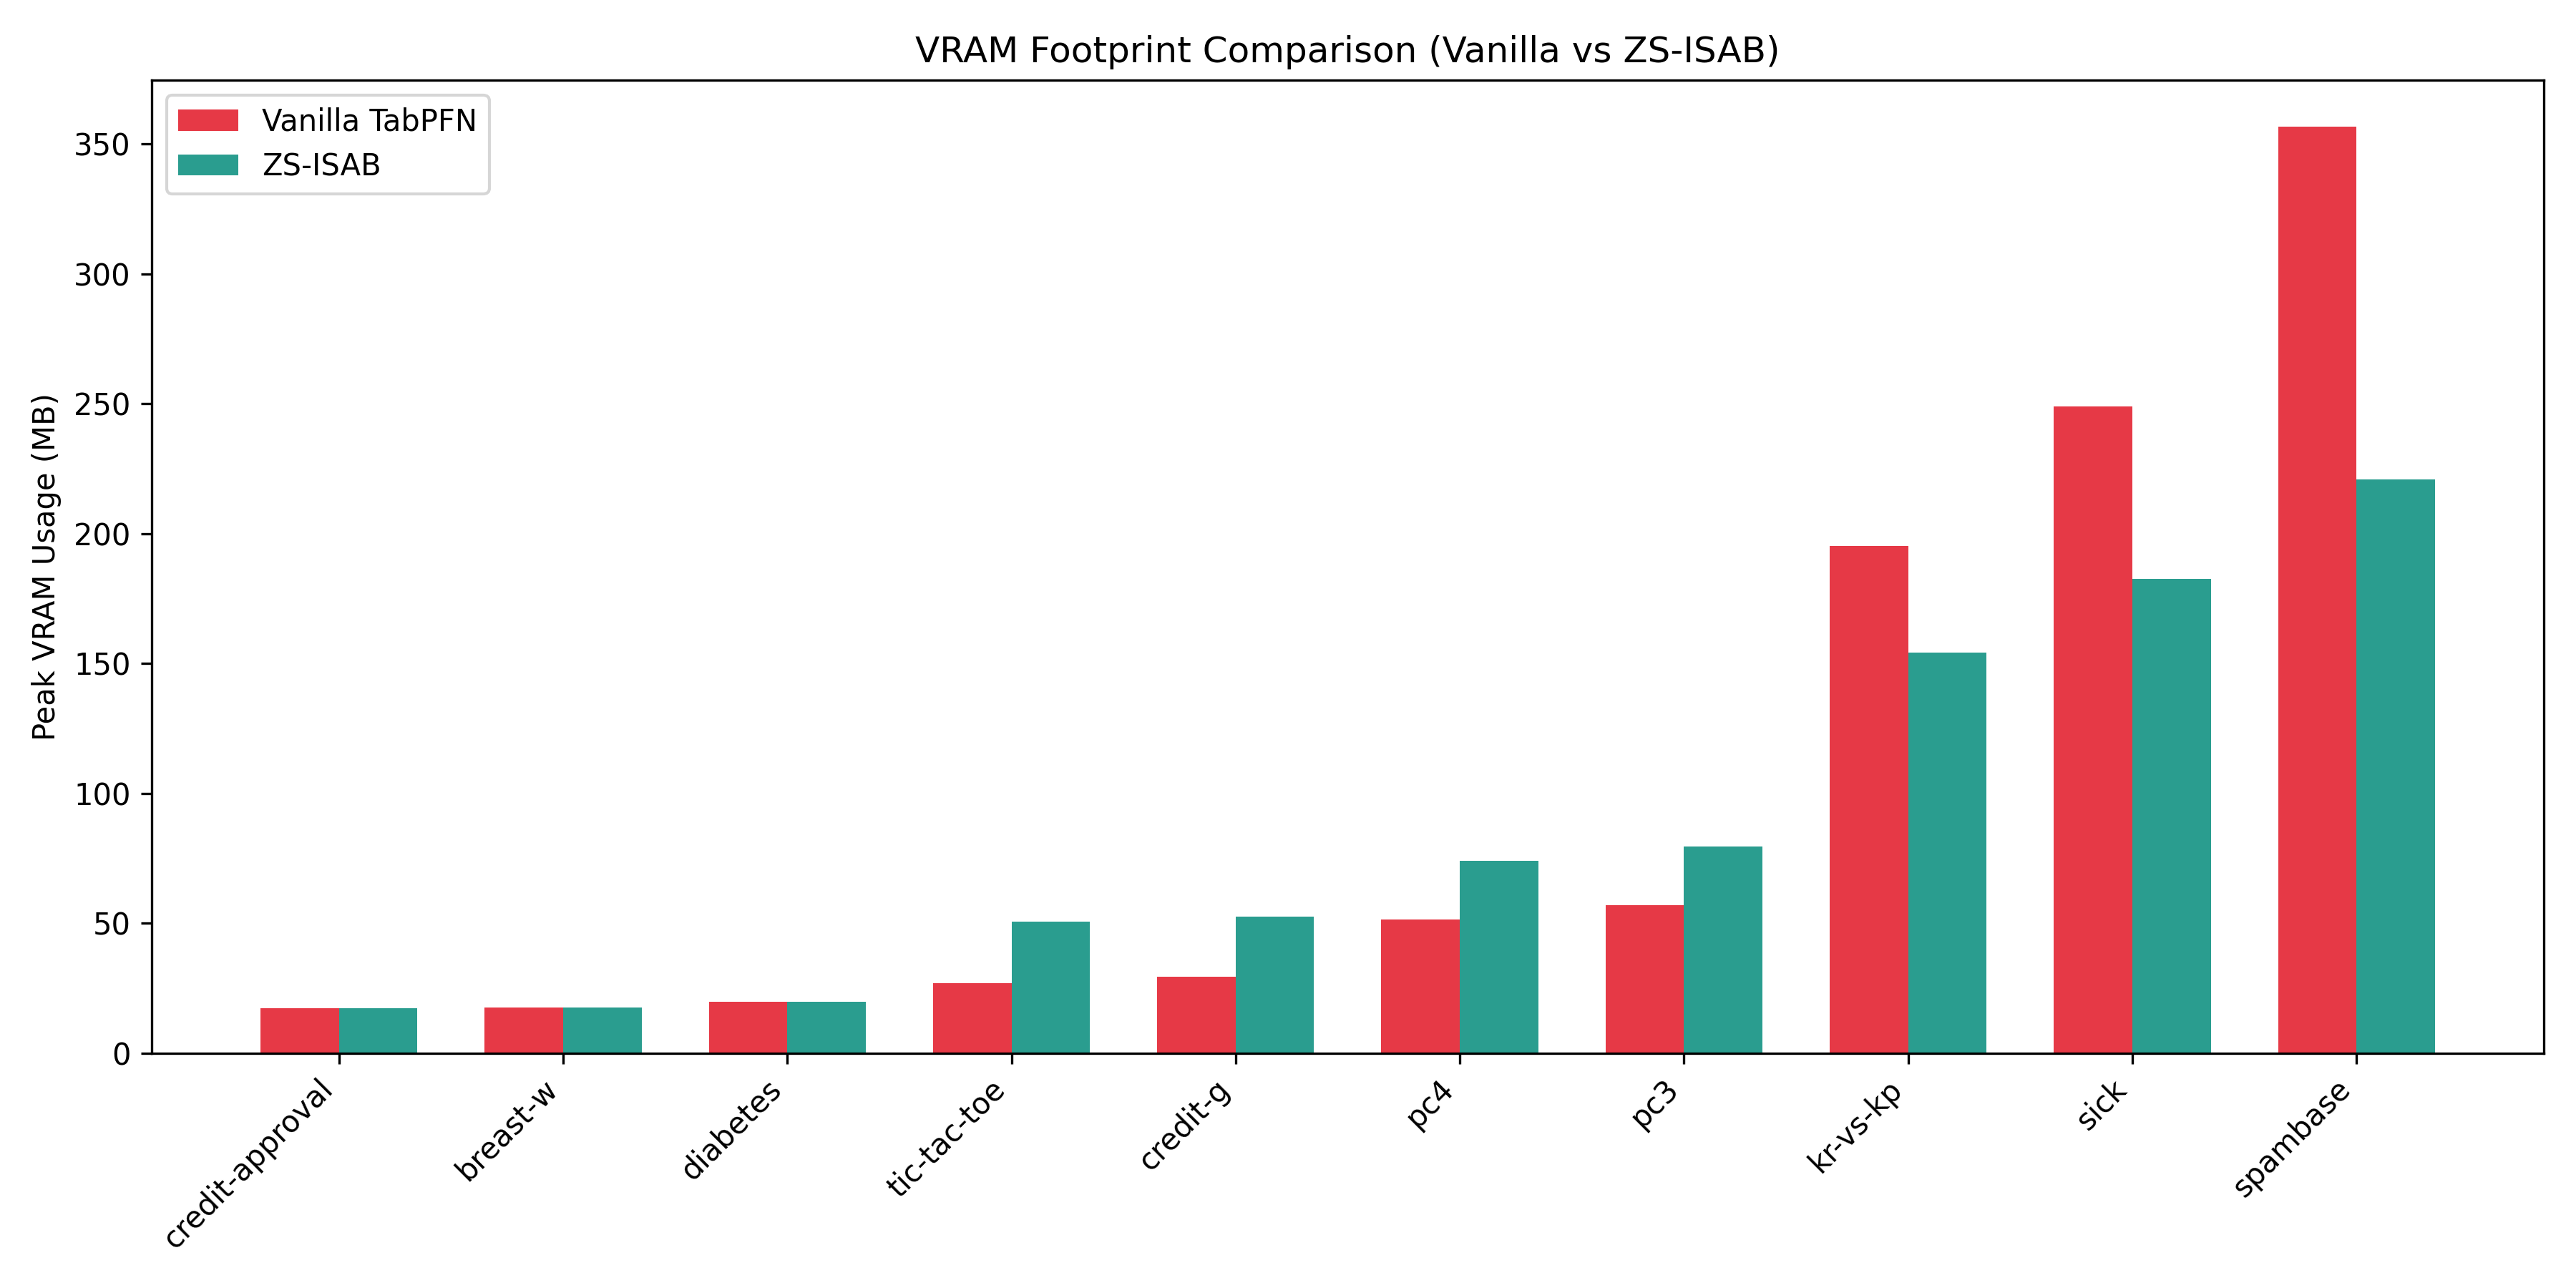
\includegraphics[width=\textwidth]{vram_comparison.png}
        \caption{Peak GPU memory scaling. Exact-attention baseline (vanilla TabPFN) grows quadratically and OOMs at $N \approx 16{,}384$. ZS-ISAB peak VRAM is constant, bounded by chunk size $B$ and prototype count $M$.}
        \label{fig:vram}
    \end{minipage}\hfill
    \begin{minipage}{0.48\textwidth}
        \centering
        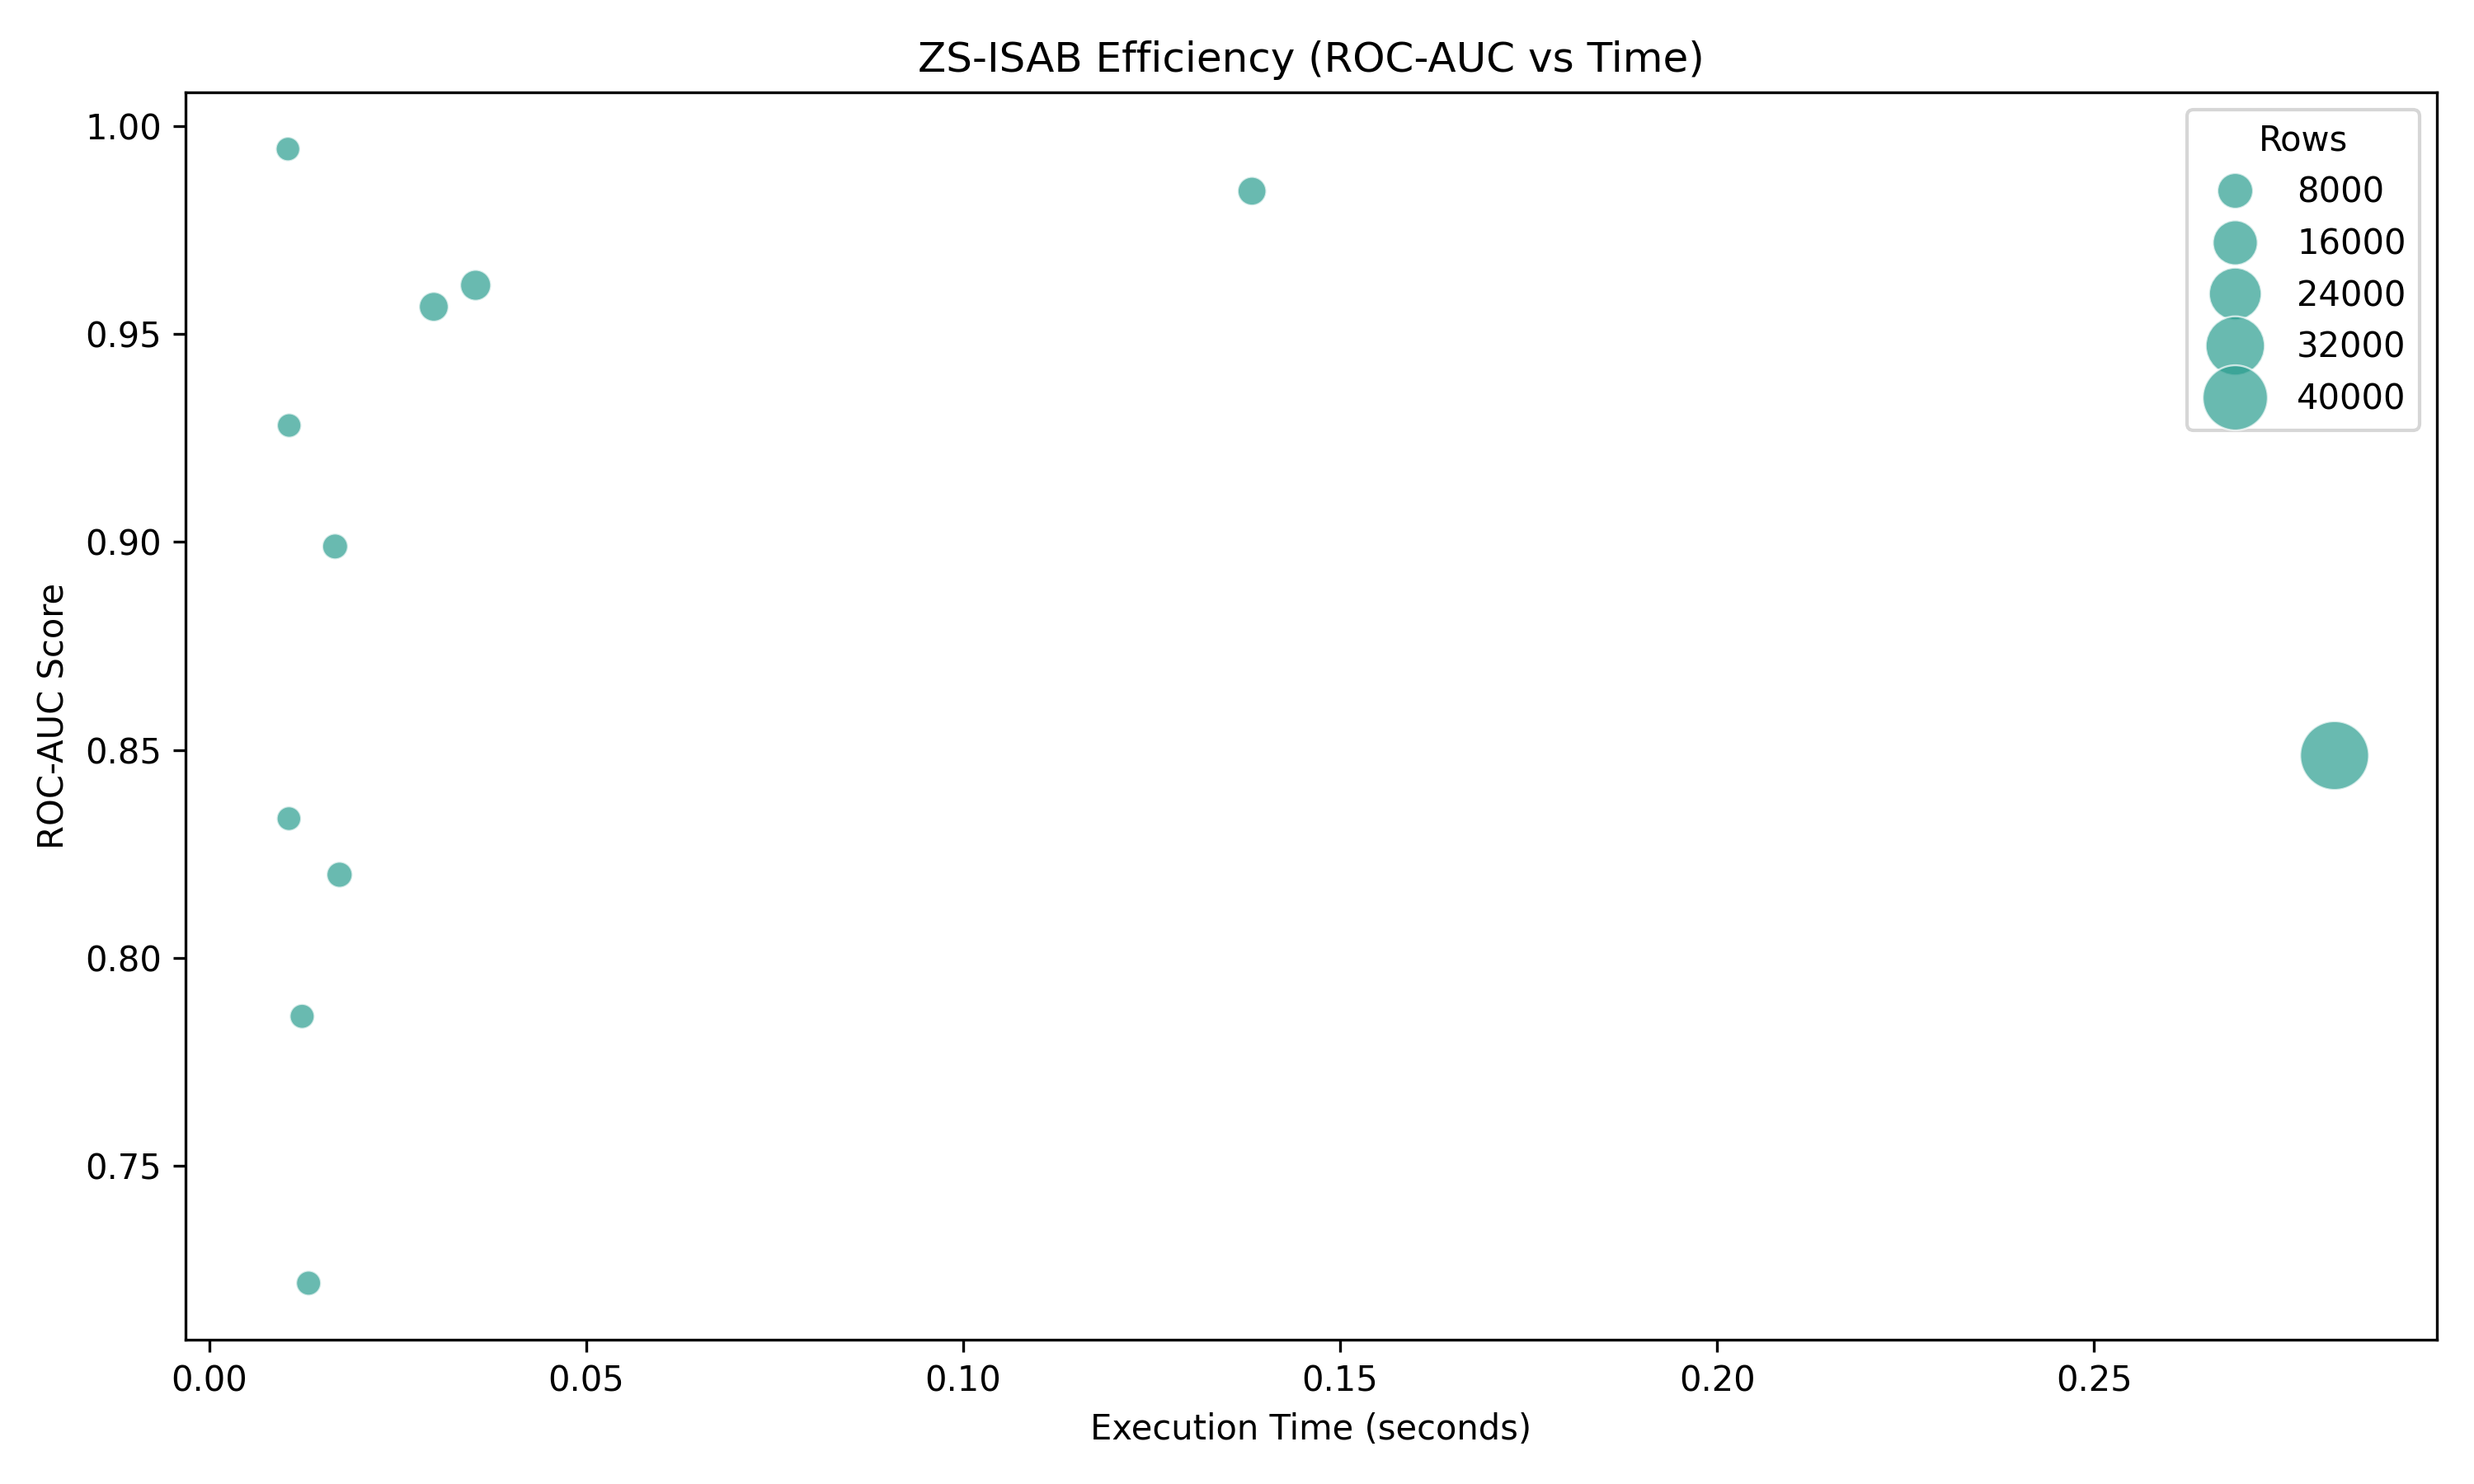
\includegraphics[width=\textwidth]{accuracy_efficiency.png}
        \caption{ROC AUC versus total wall-clock time across datasets. ZS-ISAB occupies the high-accuracy, low-time region (top-left). TabICL has comparable accuracy but higher and more variable latency.}
        \label{fig:accuracy_eff}
    \end{minipage}
\end{figure}

%------------------------------------------------------------
\subsection{Extreme Context Stress Test}
%------------------------------------------------------------

To establish an upper bound on context capacity, we ran a binary search on synthetic causal datasets of increasing $N$ on an Ubuntu server with an NVIDIA RTX 3090 Ti (24\,GB VRAM, 64\,GB system RAM). Vanilla TabPFN failed at $N = 16{,}384$. ZS-ISAB successfully completed inference up to $N = 1{,}257{,}500$ rows in 8.9\,s of execution time. At this scale the physical bottleneck is system RAM capacity, not GPU VRAM. The scaling multiplier is $1{,}257{,}500 / 16{,}384 = 76.8\times$.

On the \textit{ldpa} dataset ($N = 164{,}860$ rows, 7 features) ZS-ISAB achieves ROC AUC 0.986 in 42.7\,s of test inference. TabICL required 12{,}585.6\,s (3.5 hours) on the same dataset and achieved a lower AUC of 0.510.

%=============================================================
\section{Discussion}
%=============================================================

\textbf{Where ZS-ISAB wins.}
The largest accuracy gains over TabICL occur on multiclass datasets with many classes, such as \textit{ldpa} (+0.476 AUC) and \textit{vowel} (+0.433 AUC), and on large-row datasets where TabICL's $\mathcal{O}(N^2)$ attention degrades performance or causes timeouts. Gains over TabDPT are more distributed, with the largest margins on datasets like \textit{madelon} (+0.224 AUC) and \textit{philippine} (+0.175 AUC) where the diffusion-based prediction model appears to underfit.

\textbf{Where ZS-ISAB loses.}
The largest losses relative to TabICL occur on small datasets with fewer than 200 rows, such as \textit{visualizing\_livestock} ($-$0.227 AUC) and \textit{haberman} ($-$0.049 AUC). At very small $N$, the prototype-based approximation loses some of the fine-grained token interaction that exact attention can capture.

\textbf{Trade-offs: Training Time and Accuracy vs HPO.}
While ZS-ISAB drastically reduces inference (test) time, it incurs a one-time \emph{training time overhead} compared to standard zero-shot models. In the fit phase, ZS-ISAB must compute the prototype accumulation over all rows (Stage 2), taking roughly 20--40\,s on the largest datasets (Figure~\ref{fig:scatter_time}). Consequently, for small data where total runtime is under a second, this overhead makes it slower overall. 
Furthermore, while ZS-ISAB operates zero-shot, its accuracy was compared against deeply tuned baseline models (XGBoost, CatBoost, RandomForest) over 15,933 HPO trials. ZS-ISAB achieves a mean accuracy of 0.790, beating HPO-tuned RandomForest (0.776) and LightGBM (0.760), but falling slightly short of HPO-tuned XGBoost (0.824). This reflects the trade-off of using a foundation model: immediate competitive performance without the computational cost of running hyperparameter sweeps, though deeply-tuned classical models maintain a slight edge on axis-aligned non-linear boundaries.

\begin{figure}[htbp]
    \centering
    \begin{minipage}{0.48\textwidth}
        \centering
        \includegraphics[width=\textwidth]{scatter_time.png}
        \caption{Train vs Test Time Trade-off. ZS-ISAB trades a modest, fixed prototype accumulation time during training for massively faster, flat test time.}
        \label{fig:scatter_time}
    \end{minipage}\hfill
    \begin{minipage}{0.48\textwidth}
        \centering
        \includegraphics[width=\textwidth]{bar_accuracy.png}
        \caption{Mean Accuracy across 81 TabZilla datasets. ZS-ISAB (Zero-Shot) outperforms HPO-tuned RandomForest and LightGBM, trailing only XGBoost and CatBoost.}
        \label{fig:bar_accuracy}
    \end{minipage}
\end{figure}

\textbf{Relation to TabPFN v3.}
TabPFN v3 \citep{hollmann2025tabpfn3} achieves large-context scaling through native architectural changes and retraining, including reduced KV-cache and its own chunking mechanism. ZS-ISAB achieves comparable context ranges without retraining. The two approaches are complementary: ZS-ISAB can be applied to any existing TabPFN checkpoint including v2 and earlier versions without access to training infrastructure or H100-class hardware.

\textbf{Limitations.}
ZS-ISAB is restricted to classification tasks supported by the underlying TabPFN model. The prototype count $M$ and chunk size $B$ are fixed hyperparameters not optimized per dataset. The current evaluation covers 186 of 192 planned datasets; six large datasets are still running at the time of submission. Performance on regression tasks has not been evaluated.

%=============================================================
\section{Conclusion}
%=============================================================

We presented Zero-Shot ISAB (ZS-ISAB), a drop-in attention wrapper that extends pre-trained tabular transformers to linear-complexity inference without retraining. The method combines Seeded Anchor Selection, which avoids prototype norm compression by drawing anchors from real training rows; an Online Softmax Accumulator, which computes exact cross-attention between anchors and the full training set in bounded memory; and a Zero-Shot Attention Mask, which prevents test labels from leaking into prototype construction.

On 186 datasets from the TabZilla benchmark, ZS-ISAB achieves a mean ROC AUC of 0.927 across 141 full-comparison datasets, leads on 68.8\% of those datasets, and is the only model producing predictions on 26 additional datasets where exact-attention baselines run out of memory. It extends the usable context of TabPFN from 16{,}384 to over 1{,}257{,}500 rows --- a 76.8$\times$ increase --- while keeping peak GPU memory constant.

We thank the developers of the TabZilla benchmark suite for the evaluation infrastructure. All baseline benchmark experiments were conducted on an NVIDIA RTX 3090 Ti (24\,GB VRAM, 64\,GB system RAM) server. Even at peak scale, ZS-ISAB did not approach the hardware memory limits. We thank the authors of TabICL and TabDPT for making their implementations publicly available.

\bibliography{main}
\bibliographystyle{tmlr}

\input{assets/appendix.tex}

\end{document}
